\documentclass[10pt,journal,compsoc]{IEEEtran}
\usepackage{graphicx}
\usepackage{amsmath}
\usepackage{hyperref}
\usepackage{url}
\usepackage{booktabs}
\usepackage{multirow}
\usepackage{cite}
\usepackage{listings}
\usepackage{xcolor}
\usepackage{tikz}
\usepackage{wrapfig}
\usepackage{dblfloatfix}
\usetikzlibrary{arrows.meta, shapes.geometric, positioning, shapes.multipart}
\lstset{
	basicstyle=\ttfamily\small,
	breaklines=true,
	frame=single,
	backgroundcolor=\color{gray!5},
	keywordstyle=\color{blue}
}


% --- Corpus scale ---
\newcommand{\TotalDocs}{120,905}
\newcommand{\EPUBFiles}{74,549}
\newcommand{\ArXivDocs}{46,356}
\newcommand{\EpubTaggedDocs}{36,524}
\newcommand{\TotalPassages}{22,129,285}
\newcommand{\TotalPassagesShort}{22 million}
\newcommand{\corpussize}{82.608 GB}

% --- Tag vocabulary ---
\newcommand{\NumTags}{4,091}
\newcommand{\NumTagsAblation}{4,091}
\newcommand{\RawTags}{42,915}
\newcommand{\ISBNRawTags}{19,762}
\newcommand{\EPUBRawTags}{22,180}
\newcommand{\ArXivRawTags}{157}
\newcommand{\JunkTagsRemoved}{3,529}
\newcommand{\SingletonTagPct}{59.5}
\newcommand{\SemanticMergeIn}{37,684}
\newcommand{\SemanticMergeOut}{4{,}091}
\newcommand{\SimilarityThreshold}{0.85}
\newcommand{\FrequencyPruneMin}{5}

% --- Label sources (tag assignment counts) ---
\newcommand{\TagsTotalAssignments}{361{,}180}
\newcommand{\TagsEPUBMeta}{147{,}448}
\newcommand{\TagsEPUBMetaPct}{40.8}
\newcommand{\TagsISBN}{103{,}715}
\newcommand{\TagsISBNPct}{28.7}
\newcommand{\TagsArXiv}{93{,}315}
\newcommand{\TagsArXivPct}{25.8}
\newcommand{\TagsPaths}{15{,}170}
\newcommand{\TagsPathsPct}{4.2}
\newcommand{\TagsLLM}{1{,}532}
\newcommand{\TagsLLMPct}{0.4}

% --- Document-level label source breakdown (pie chart pct) ---
\newcommand{\PctArXivLabels}{78.4}
\newcommand{\PctISBNLabels}{11.4}
\newcommand{\PctPredictedLabels}{7.1}
\newcommand{\PctLLMLabels}{1.3}

% --- Gold / Silver label counts ---
\newcommand{\GoldLabelDocs}{82,880}
\newcommand{\SilverLabelDocs}{234}

% --- EPUB conversion ---
\newcommand{\EPUBSuccessRate}{100}
\newcommand{\EPUBPendingRate}{0}
\newcommand{\EPUBFailRate}{0}

% --- Training: Stage 1 ---
\newcommand{\ContrastivePairs}{1,598,044}
\newcommand{\PosPairs}{800,000}
\newcommand{\NegPairs}{800,000}
\newcommand{\StageOneEpochs}{1}
\newcommand{\StageOneBatch}{128}
\newcommand{\StageOneLR}{2\times10^{-5}}

% --- Training: Stage 2 ---
\newcommand{\StageTwoEpochs}{128}
\newcommand{\StageTwoBatch}{16384}
\newcommand{\StageTwoLR}{1\times10^{-3}}
\newcommand{\MLPHiddenDim}{512}
\newcommand{\MLPDropout}{0.2}
\newcommand{\EncoderDim}{384}

% --- Evaluation: main results (combined corpus, passage-level) ---
\newcommand{\MicroF}{0.485}
\newcommand{\MacroF}{0.434}
\newcommand{\HammingL}{0.0011}
\newcommand{\Throughput}{1,401}
% --- ArXiv-only subset (clean document-level labels) ---
\newcommand{\ArXivMicroF}{0.76}
\newcommand{\ArXivMacroF}{0.41}

% --- Ablation results (ArXiv-only subset) ---
\newcommand{\AblMLPOptMicro}{0.76}
\newcommand{\AblMLPOptMacro}{0.41}
\newcommand{\AblOvROptMicro}{0.72}
\newcommand{\AblOvROptMacro}{0.35}
\newcommand{\AblMLPGlobalMicro}{0.73}
\newcommand{\AblMLPGlobalMacro}{0.38}
\newcommand{\AblOvRGlobalMicro}{0.69}
\newcommand{\AblOvRGlobalMacro}{0.30}
\newcommand{\AblEnsOptMicro}{0.75}
\newcommand{\AblEnsOptMacro}{0.40}
\newcommand{\GlobalThreshold}{0.375}

% --- Dataset split ---
\newcommand{\TrainSplitPct}{80}
\newcommand{\ValSplitPct}{10}
\newcommand{\TestSplitPct}{10}

% --- Hardware ---
\newcommand{\CPUThreads}{128}
\newcommand{\EPUBWorkers}{96}
\newcommand{\MMAPSize}{32}
\newcommand{\CacheSize}{8}
\newcommand{\DBSize}{120}

% --- Tag name length threshold ---
\newcommand{\TagMaxChars}{60}

% --- pos_weight ablation ---
\newcommand{\EPUBChunkMicroF}{0.485}
\newcommand{\EPUBChunkMacroF}{0.434}
\newcommand{\EPUBChunkHammingL}{0.0011}
\newcommand{\PosWeightMicroF}{0.10}
\newcommand{\NoPosWeightEpochFour}{0.33}
\newcommand{\PosWeightMax}{100}
\newcommand{\PosWeightDelta}{0.385}
\newcommand{\EPUBLossStart}{0.07}
\newcommand{\EPUBLossFinal}{0.006}
\newcommand{\EPUBOptThreshold}{0.225}
\newcommand{\EPUBOptThresholdF}{0.516}
% --- Ranking metrics ---
\newcommand{\HitRateOne}{0.640}
\newcommand{\HitRateFive}{0.848}
\newcommand{\HitRateTen}{0.906}
\newcommand{\PrecisionFive}{0.394}
\newcommand{\NDCGTen}{0.626}
\newcommand{\MAPScore}{0.558}
% --- Per-bucket F1 ---
\newcommand{\BucketHead}{0.441}
\newcommand{\BucketMid}{0.365}
\newcommand{\BucketTail}{0.079}
\newcommand{\BucketRare}{0.000}
% --- Tag coverage ---
\newcommand{\CovFiveZero}{1{,}554}
\newcommand{\CovThreeZero}{2{,}885}
\newcommand{\CovOneZero}{3{,}868}
\newcommand{\CovAny}{4{,}044}
% --- Label cardinality ---
\newcommand{\PredCardinality}{2.95}
\newcommand{\GTCardinality}{5.79}
\newcommand{\CardinalityRatio}{0.51}
% --- Validation sample count ---
\newcommand{\ValSamples}{1{,}191{,}047}


\begin{document}
	
	\title{High-Performance Document Tagging: An Extension of the SetFit Framework}
	
	\author{Townsend Southard Pantano%
		\IEEEcompsocitemizethanks{\IEEEcompsocthanksitem E-mail: tgsoutha@syr.edu}}
	
	\IEEEtitleabstractindextext{%
		\begin{abstract}
This paper presents a production-scale multi-label tagging pipeline built on SetFit, classifying \TotalDocs{} scientific documents across \NumTags{} categories. Gold-standard ISBN and ArXiv metadata are combined with LLM-distilled silver labels to train a two-stage model: contrastive fine-tuning of \texttt{all-MiniLM-L6-v2} followed by a deep MLP head. On the combined passage-level corpus, the system achieves Micro-F1 \MicroF{}, Macro-F1 \MacroF{}, and Hit@5 \HitRateFive{} at \Throughput{}+ passages per second; on the clean ArXiv-only subset, Micro-F1 reaches \ArXivMicroF{}. Ablation confirms MLP head and per-tag threshold optimization improve over standard SetFit baselines, and reveals that \texttt{pos\_weight} correction catastrophically suppresses learning under noisy inherited labels.
		\end{abstract}
}
	
	\maketitle
	\IEEEdisplaynontitleabstractindextext
	%\IEEEpeerreviewmaketitle
	
	\section{Introduction}
	\IEEEPARstart{M}{ulti-label classification} (MLC) offers a scalable solution to efficient document search, but traditional approaches struggle with high-cardinality label spaces and the cold-start problem in sparsely annotated domains.
	
	The \textbf{Sentence Transformer Fine-Tuning (SetFit)} framework \cite{tunstall_efficient_2022} addresses the data-efficiency problem by decoupling contrastive representation learning from classifier training. However, SetFit has been evaluated primarily on low-cardinality benchmarks (5 to 20 labels), and its default logistic regression head may not suffice when the label space spans thousands of categories. In this paper, I present a production-scale extension of SetFit to a \TotalDocs{}-document corpus with over \NumTagsAblation{} curated labels, replacing the standard classification head with a deep MLP trained using \texttt{BCEWithLogitsLoss}. Evaluated on the full passage-level corpus with document-inherited labels, the system achieves Micro-F1 of \MicroF{} and Hit Rate@5 of \HitRateFive{} at \Throughput{} passages per second; on the ArXiv-only subset with clean document-level labels, Micro-F1 reaches \ArXivMicroF{}. I also show that naive \texttt{pos\_weight} amplification catastrophically suppresses learning under noisy label regimes while the architecture itself remains sound.
	
	\section{Contributions}
	This work makes the following contributions beyond prior research:
	\begin{enumerate}
		\item \textbf{Scaling SetFit to high-cardinality multi-label classification.}
		The original SetFit framework \cite{tunstall_efficient_2022} was evaluated on
		5--20 labels; I extend it to \NumTagsAblation{} simultaneous tags, demonstrating that the
		contrastive-then-classify paradigm remains effective at this scale.
		
		\item \textbf{Hybrid gold/silver label synthesis with provenance tracking.}
		Five label streams (EPUB metadata, filesystem structure, ISBN subject headings,
		ArXiv categories, and LLM-distilled labels) are unified in a single schema that
		tracks source and confidence. A SQLite trigger automatically replaces
		low-confidence predictions when higher-fidelity labels arrive.
		
		\item \textbf{Semantic label reduction.} Using an embedding model pre-trained
		on the corpus, tens of thousands of raw labels are pruned to only those carrying
		the greatest semantic weight.
		
		\item \textbf{Deep MLP classification head for SetFit.} Replacing the standard
		logistic regression head with a three-layer MLP (\EncoderDim{}$\rightarrow$\MLPHiddenDim{}$\rightarrow$\NumTagsAblation{}) yields a 3--4
		point Micro-F1 gain (Table~\ref{tab:ablation}), confirming that non-linear
		capacity benefits high-cardinality label mapping.
		
		\item \textbf{Per-tag threshold optimization.} Sweeping decision boundaries
		independently for each of the \NumTagsAblation{} tags on the validation set yields an
		additional 3-point Micro-F1 gain over a fixed global threshold, with the
		largest impact on medium-frequency tags.
		
		\item \textbf{Analysis of \texttt{pos\_weight} failure under label noise.} I demonstrate that naive class-imbalance correction via \texttt{pos\_weight} catastrophically suppresses learning (Micro-F1 $\approx$ \PosWeightMicroF{}) when applied to passage-level labels inherited from document-level annotations. Removing \texttt{pos\_weight} recovers Micro-F1 to \MicroF{}, a \PosWeightDelta{}-point improvement. The gap between the clean ArXiv-only subset (\ArXivMicroF{}) and the full corpus (\MicroF{}) quantifies the cost of label noise inherent in document-inherited passage labels.
	\end{enumerate}
	
	\section{Related Work}
	
	\subsection{Multi-Label Classification at Scale}
	Multi-label classification (MLC) has evolved from flat one-vs-rest schemes toward
	architectures exploiting label correlations. Early TF-IDF approaches scale poorly
	beyond a few hundred labels due to feature sparsity \cite{abbas_automated_2023},
	while BERT-based fine-tuning improves performance but remains computationally
	prohibitive when the label space exceeds thousands of categories and annotated data
	is scarce \cite{minilm}. Established large-scale systems such as PubMed's MeSH
	indexer rely on domain-specific ontologies and significant human curation, limiting
	portability to new corpora.
	
	Menke et al.\ demonstrated that \texttt{BCEWithLogitsLoss} with independent sigmoid
	outputs outperforms softmax-based approaches for multi-label publication tagging when
	label co-occurrence is common \cite{menke_publication_2025}. This work extends that
	finding to a substantially larger label space (\NumTagsAblation{} tags) within the SetFit paradigm.
	
	\subsection{SetFit and Few-Shot Learning}
	Tunstall et al.\ introduced SetFit as an efficient alternative to prompt-based
	few-shot learning, decoupling contrastive representation learning from classifier
	training and achieving competitive performance against GPT-3 using orders of magnitude
	less data \cite{tunstall_efficient_2022}. However, original SetFit evaluations were
	limited to low-cardinality tasks (5--20 labels), and the default logistic regression
	head may not capture non-linear dependencies in high-cardinality settings. This work
	addresses that gap by substituting a deep MLP head and scaling contrastive pair
	generation to \ContrastivePairs{} examples across over \NumTagsAblation{} categories.
	
	\subsection{Knowledge Distillation for Label Augmentation}
	Knowledge distillation from large language models has emerged as a practical strategy
	for generating training labels where human annotation is expensive
	\cite{hinton_distilling_2015}. I adopt a hybrid strategy combining authoritative
	metadata (ISBN subjects and ArXiv categories) with silver-standard labels from a
	locally hosted LLM, creating a label hierarchy that explicitly tracks provenance
	and confidence.
	
	\section{NLP Pipeline and Experimental Setup}
	I have architected the system as a modular suite of Python-based processing tiers
	designed to feed the two-stage SetFit training loop (Fig.\ \ref{fig:file_pipeline}).
	
	\begin{figure*}[!t]
		\centering
		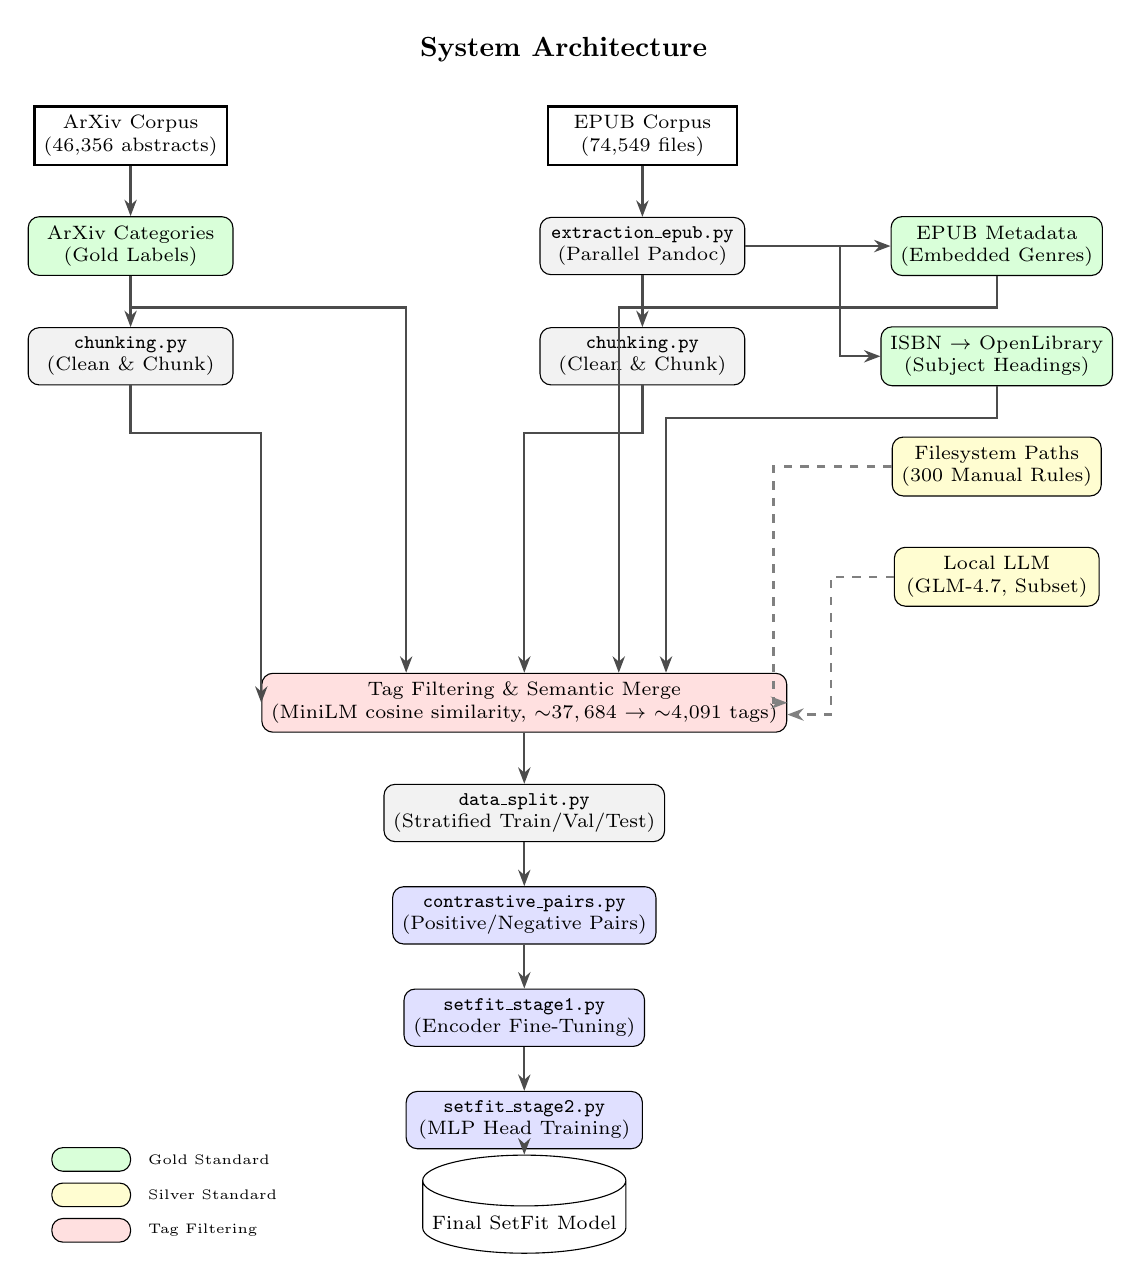
\begin{tikzpicture}[
			node distance=1.0cm and 1.8cm,
			every node/.style={fill=white, font=\scriptsize, align=center},
			proc/.style={draw, rounded corners, fill=gray!10, minimum width=2.6cm, minimum height=0.7cm},
			gold/.style={draw, rounded corners, fill=green!15, minimum width=2.6cm, minimum height=0.7cm},
			silver/.style={draw, rounded corners, fill=yellow!18, minimum width=2.6cm, minimum height=0.7cm},
			filter/.style={draw, rounded corners, fill=red!12, minimum width=5.0cm, minimum height=0.7cm},
			train/.style={draw, rounded corners, fill=blue!12, minimum width=3.0cm, minimum height=0.7cm},
			src/.style={draw, rectangle, fill=white, minimum width=2.4cm, minimum height=0.7cm, thick},
			arr/.style={-{Stealth[scale=0.9]}, thick, color=black!70},
			darr/.style={-{Stealth[scale=0.9]}, thick, dashed, color=black!50}
			]
			
			% Title at top of figure
			\node [font=\normalsize\bfseries, fill=none] at (5.5, 1.1) {System Architecture};
			
			\node (arxiv) [src] at (0, 0)     {ArXiv Corpus\\(\ArXivDocs{} abstracts)};
			\node (epub)  [src] at (6.5, 0)   {EPUB Corpus\\(\EPUBFiles{} files)};
			
			\node (arxiv_tags)  [gold] at (0, -1.4)  {ArXiv Categories\\(Gold Labels)};
			\node (arxiv_chunk) [proc] at (0, -2.8)  {\texttt{chunking.py}\\(Clean \& Chunk)};
			
			\node (extract)    [proc] at (6.5, -1.4) {\texttt{extraction\_epub.py}\\(Parallel Pandoc)};
			\node (epub_chunk) [proc] at (6.5, -2.8) {\texttt{chunking.py}\\(Clean \& Chunk)};
			
			\node (epubmeta) [gold]   at (11.0, -1.4) {EPUB Metadata\\(Embedded Genres)};
			\node (isbn)     [gold]   at (11.0, -2.8) {ISBN $\rightarrow$ OpenLibrary\\(Subject Headings)};
			\node (paths)    [silver] at (11.0, -4.2) {Filesystem Paths\\(300 Manual Rules)};
			\node (llm)      [silver] at (11.0, -5.6) {Local LLM\\(GLM-4.7, Subset)};
			
			\node (tagmerge) [filter] at (5.0, -7.2)
			{Tag Filtering \& Semantic Merge\\(MiniLM cosine similarity, ${\sim}\SemanticMergeIn{}$ $\rightarrow$ ${\sim}\SemanticMergeOut{}$ tags)};
			
			\node (split)  [proc,  minimum width=3.0cm] at (5.0, -8.6)
			{\texttt{data\_split.py}\\(Stratified Train/Val/Test)};
			\node (pairs)  [train] at (5.0, -9.9)
			{\texttt{contrastive\_pairs.py}\\(Positive/Negative Pairs)};
			\node (stage1) [train] at (5.0, -11.2)
			{\texttt{setfit\_stage1.py}\\(Encoder Fine-Tuning)};
			\node (stage2) [train] at (5.0, -12.5)
			{\texttt{setfit\_stage2.py}\\(MLP Head Training)};
			\node (model)  [draw, cylinder, shape border rotate=90, aspect=0.25]
			at (5.0, -13.8) {Final SetFit Model};
			
			\draw [arr] (arxiv)       -- (arxiv_tags);
			\draw [arr] (arxiv_tags)  -- (arxiv_chunk);
			\draw [arr] (arxiv_chunk.south) -- ++(0, -0.6) -| (tagmerge.west);
			
			\draw [arr] (epub)    -- (extract);
			\draw [arr] (extract) -- (epub_chunk);
			\draw [arr] (extract.east) -- (epubmeta.west);
			\draw [arr] (extract.east) -- ++(1.2, 0) |- (isbn.west);
			\draw [arr] (epub_chunk.south) -- ++(0, -0.6) -| (tagmerge.north);
			
			\draw [arr]  (epubmeta.south) -- ++(0, -0.4) -| ([xshift=1.2cm]tagmerge.north);
			\draw [arr]  (isbn.south)     -- ++(0, -0.4) -| ([xshift=1.8cm]tagmerge.north);
			
			\draw [darr] (paths.west) -- ++(-1.5, 0) |- (tagmerge.east);
			\draw [darr] (llm.west)   -- ++(-0.8, 0) |- ([yshift=-0.15cm]tagmerge.east);
			
			\draw [arr] (arxiv_tags.south) -- ++(0, -0.4) -| ([xshift=-1.5cm]tagmerge.north);
			
			\draw [arr] (tagmerge) -- (split);
			\draw [arr] (split)    -- (pairs);
			\draw [arr] (pairs)    -- (stage1);
			\draw [arr] (stage1)   -- (stage2);
			\draw [arr] (stage2)   -- (model);
			
			\begin{scope}[shift={(-0.5, -13.0)}]
				\node [gold,   minimum width=1.0cm, minimum height=0.3cm, font=\tiny] at (0, 0) {};
				\node [anchor=west, font=\tiny] at (0.6, 0) {Gold Standard};
				\node [silver, minimum width=1.0cm, minimum height=0.3cm, font=\tiny] at (0, -0.45) {};
				\node [anchor=west, font=\tiny] at (0.6, -0.45) {Silver Standard};
				\node [filter, minimum width=1.0cm, minimum height=0.3cm, font=\tiny] at (0, -0.9) {};
				\node [anchor=west, font=\tiny] at (0.6, -0.9) {Tag Filtering};
			\end{scope}
			
		\end{tikzpicture}
		\caption{ArXiv categories serve directly as gold labels. EPUB documents are tagged via four sources: embedded OPF metadata (gold), ISBN-to-OpenLibrary subject lookups (gold), filesystem path heuristics (silver), and local LLM distillation (silver, dashed). All raw tags pass through a semantic merge stage that uses MiniLM cosine similarity to consolidate ${\sim}\SemanticMergeIn{}$ tag variants into ${\sim}\SemanticMergeOut{}$ canonical categories before stratified splitting and SetFit training.}
		\label{fig:file_pipeline}
	\end{figure*}
	
	\subsection{Dataset Composition}
	The corpus consists of \TotalDocs{} documents drawn from two sources: \EPUBFiles{}
	EPUB files extracted from a heterogeneous digital library and \ArXivDocs{} ArXiv
	abstracts ingested from the Kaggle ArXiv metadata snapshot. Table \ref{tab:dataset}
	summarizes the dataset composition.
	
	\begin{table}[htbp]
		\centering
		\caption{Dataset and label source summary.}
		\label{tab:dataset}
		\begin{tabular}{@{}lr@{}}
			\toprule
			\textbf{Metric} & \textbf{Value} \\
			\midrule
			Total documents processed & \TotalDocs{} \\
			Passages (chunks) generated & \TotalPassages{} \\
			Unique tags (vocabulary) & \NumTags{} \\
			Gold labels (ISBN + ArXiv) & \GoldLabelDocs{} docs \\
			Silver labels (LLM) & \SilverLabelDocs{} docs \\
			Corpus Size {GB} & \corpussize{}\\
			\bottomrule
		\end{tabular}
	\end{table}
	
\subsection{Tag Acquisition}

Extracting useful tags from tens of thousands of documents required multiple sourcing methods and a reduction pipeline to retain only semantically valuable tags.

ArXiv tags were the simplest to acquire: \ArXivRawTags{} unique tags across \ArXivDocs{} documents. EPUB tags required four additional methods:

\begin{itemize}
	\item \textbf{ISBNs:} EPUBs with attached ISBNs were looked up against the OpenLibrary database, yielding \ISBNRawTags{} unique tags.
	\item \textbf{EPUB Metadata:} Parsing embedded XML metadata extracted \EPUBRawTags{} additional tags.
	\item \textbf{File Paths:} Filesystem organization (e.g., ``Physics'', ``Computer Science'' folders) provided coarse but useful signal.
	\item \textbf{LLM Tagging:} A locally hosted GLM 4.7 generated tags for untagged documents; limited to a small subset due to computational cost.
\end{itemize}

This yielded \RawTags{} raw tags, most of which were unusable: $\SingletonTagPct\%$ occurred only once, and EPUB metadata frequently leaked ISBNs and other noise. Label assignments by source are shown in Fig.\ \ref{fig:tag_source_dist}: EPUB metadata (\TagsEPUBMetaPct{}\%), ISBN (\TagsISBNPct{}\%), ArXiv (\TagsArXivPct{}\%), file paths (\TagsPathsPct{}\%), and LLM (\TagsLLMPct{}\%).

The vocabulary was reduced via a five-step pipeline:

\begin{enumerate}
	\item \textbf{Regex junk removal.} Discarded numeric-leading strings (leaked ISBNs), BISAC codes, bestseller references, format descriptors, Lexile levels, fictional character tags, and strings exceeding \TagMaxChars{} characters. Eliminated approximately \JunkTagsRemoved{} tags.
	\item \textbf{Prefix/suffix normalization.} Collapsed trivial variants by stripping \texttt{fiction\_}, \texttt{\_fiction}, and \texttt{\_general}, reducing \texttt{fiction\_romance\_general}, \texttt{romance\_fiction}, and \texttt{romance} to a single canonical form.
	\item \textbf{Semantic deduplication.} Tag names were encoded with the fine-tuned \texttt{all-MiniLM-L6-v2} encoder and merged at cosine similarity $\geq$ \SimilarityThreshold{}, capturing synonyms invisible to string matching (e.g., \texttt{science\_fiction}/\texttt{scifi}, \texttt{biography\_autobiography}/\texttt{biographies}).
	\item \textbf{Frequency pruning.} Tags with fewer than \FrequencyPruneMin{} document-level occurrences were removed as insufficient for contrastive training.
	\item \textbf{Cross-source deduplication.} Where multiple sources assigned the same canonical tag to a document, only the highest-confidence assignment was retained.
\end{enumerate}

This pipeline reduced the vocabulary from \RawTags{} raw tags to \NumTagsAblation{} canonical categories, each semantically distinct and sufficiently supported.
	
	\begin{figure}[htbp]
		\centering
		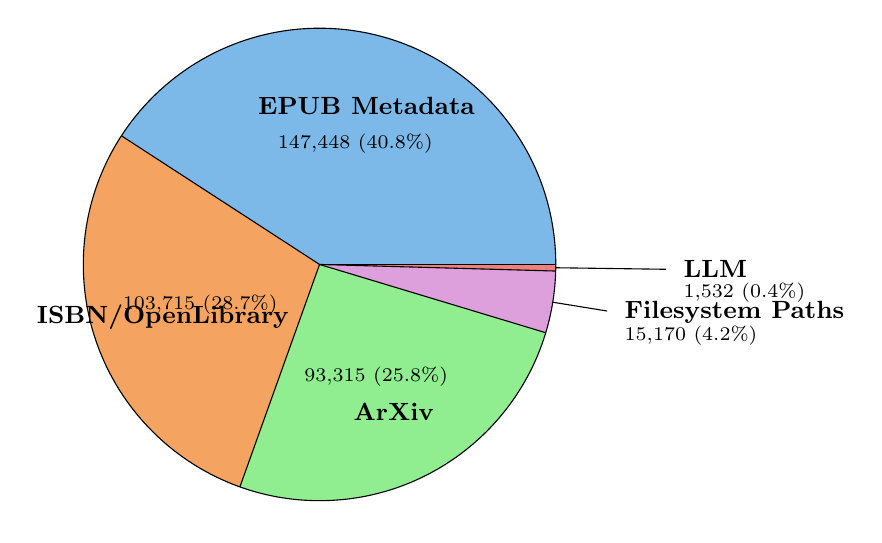
\begin{tikzpicture}
			\def\radius{3.0}
			\definecolor{cepub}{HTML}{7CB9E8}
			\definecolor{cisbn}{HTML}{F4A460}
			\definecolor{carxiv}{HTML}{90EE90}
			\definecolor{cpath}{HTML}{DDA0DD}
			\definecolor{cllm}{HTML}{F08080}
			
			\fill[cepub]   (0,0) -- (0:\radius) arc (0:147.0:\radius) -- cycle;
			\fill[cisbn]   (0,0) -- (147.0:\radius) arc (147.0:250.3:\radius) -- cycle;
			\fill[carxiv]  (0,0) -- (250.3:\radius) arc (250.3:343.2:\radius) -- cycle;
			\fill[cpath]   (0,0) -- (343.2:\radius) arc (343.2:358.4:\radius) -- cycle;
			\fill[cllm]    (0,0) -- (358.4:\radius) arc (358.4:360:\radius) -- cycle;
			
			\draw (0,0) circle (\radius);
			\foreach \a in {0, 147.0, 250.3, 343.2, 358.4} {
				\draw (0,0) -- (\a:\radius);
			}
			
			\node[font=\small\bfseries] at (73.5:2.1)  {EPUB Metadata};
			\node[font=\scriptsize]     at (73.5:1.6)  {\TagsEPUBMeta{} (\TagsEPUBMetaPct{}\%)};
			
			\node[font=\small\bfseries] at (198.6:2.1) {ISBN/OpenLibrary};
			\node[font=\scriptsize]     at (198.6:1.6) {\TagsISBN{} (\TagsISBNPct{}\%)};
			
			\node[font=\small\bfseries] at (296.7:2.1) {ArXiv};
			\node[font=\scriptsize]     at (296.7:1.6) {\TagsArXiv{} (\TagsArXivPct{}\%)};
			
			\draw (350.8:\radius) -- (350.8:\radius+0.7);
			\node[anchor=west, font=\small\bfseries] at (350.8:\radius+0.8) {Filesystem Paths};
			\node[anchor=west, font=\scriptsize]      at (350.8:\radius+0.8) [yshift=-0.3cm] {\TagsPaths{} (\TagsPathsPct{}\%)};
			
			\draw (359.2:\radius) -- (359.2:\radius+1.4);
			\node[anchor=west, font=\small\bfseries] at (359.2:\radius+1.5) {LLM};
			\node[anchor=west, font=\scriptsize]      at (359.2:\radius+1.5) [yshift=-0.3cm] {\TagsLLM{} (\TagsLLMPct{}\%)};
			
		\end{tikzpicture}
		\caption{Distribution of tag assignments by source. EPUB embedded metadata and ISBN subject lookups collectively account for the number of all tag assignments, with ArXiv categories contributing \TagsArXivPct{}\%. Filesystem path heuristics and LLM-distilled labels provide supplementary coverage for documents lacking structured metadata.}
		\label{fig:tag_source_dist}
	\end{figure}
	
	\subsection{Surgical Cleaning and Semantic Noise Reduction}
	EPUB extractions via Pandoc \cite{pandoc} contain mathematical symbols, tables,
	inline citations, and structural boilerplate that degrade Sentence Transformer
	training. Cleaning proceeds in two passes within \texttt{chunking.py}.
	
	\textbf{1) Global Boilerplate Removal:} Regular expressions strip structural blocks
	(``Table of Contents,'' ``Index,'' ``Bibliography''), Pandoc artifacts
	(\texttt{\{\#id\}}, \texttt{[text]\{style\}}), and excess whitespace.
	
	\textbf{2) Local Chunk Filtering:} Each passage is evaluated against three filters:
	\begin{itemize}
		\item \textbf{Citation Density:} Passages with more than five inline citations
		are discarded to prevent overfitting to bibliographic formats.
		\item \textbf{Alphanumeric Density:} Passages below a 0.4 ratio
		$\left(\frac{\text{[a-zA-Z0-9]}}{\text{total chars}}\right)$
		are dropped as likely tables, code, or formulas.
		\item \textbf{Length:} Passages under 20 words are discarded.
	\end{itemize}
	
	\subsection{Tokenization and Overlapping Chunking Strategy}
	The \texttt{all-MiniLM-L6-v2} encoder uses a 30,522-token WordPiece vocabulary.
	Sub-word tokenization handles scientific OOV terms effectively, but the 512-token
	sequence limit requires long documents to be segmented. I use a 500-token sliding
	window with a 50-token stride, ensuring that interdisciplinary transition passages
	spanning section boundaries are fully captured in at least one context window.
	
	\subsection{Train/Validation/Test Split}
	The ArXiv portion of the dataset was split into training (\TrainSplitPct{}\%),
	validation (\ValSplitPct{}\%), and test (\TestSplitPct{}\%) partitions using
	stratified sampling by primary ArXiv category, preserving category proportions
	across splits so that evaluation is not biased by dominant fields such as
	high-energy physics or mathematics.
	
	\subsection{Training Hyperparameters}
	Table \ref{tab:hyperparams} lists the key hyperparameters for both training stages.
	
	\begin{table}[htbp]
		\centering
		\caption{Training hyperparameters.}
		\label{tab:hyperparams}
		\begin{tabular}{@{}lll@{}}
			\toprule
			\textbf{Parameter} & \textbf{Stage 1} & \textbf{Stage 2} \\
			\midrule
			Base model & all-MiniLM-L6-v2 & (frozen encoder) \\
			Contrastive pairs & \ContrastivePairs{} & n/a \\
			Loss function & CosineSimilarityLoss & BCEWithLogitsLoss \\
			Epochs & \StageOneEpochs{} & \StageTwoEpochs{} \\
			Batch size & \StageOneBatch{} & \StageTwoBatch{} \\
			Learning rate & $\StageOneLR$ (default) & $\StageTwoLR$ \\
			Hidden layer & n/a & \MLPHiddenDim{} (ReLU, Dropout=\MLPDropout{}) \\
			Optimizer & AdamW & Adam \\
			\bottomrule
		\end{tabular}
	\end{table}
	
	\section{SetFit Implementation Details}
	The core of this work is the two-stage training workflow optimized for high-cardinality multi-label classification.
	
	\subsection{Stage 1: Contrastive Embedding Refinement}
	Stage 1 fine-tunes the \texttt{all-MiniLM-L6-v2} encoder so passages sharing
	disciplinary content cluster in the \EncoderDim{}-dimensional embedding space.
	Training uses \ContrastivePairs{} deduplicated
	\emph{(passage\textsubscript{a}, passage\textsubscript{b}, similarity)} triples:
	
	\begin{itemize}
		\item \textbf{Positive pairs} ($sim=1.0$): \PosPairs{} pairs from documents
		sharing at least one canonical tag, sampled in descending tag-frequency order
		so rare tags contribute at least one pair.
		\item \textbf{Negative pairs} ($sim=0.0$): \NegPairs{} pairs from documents
		with zero tag overlap, drawn uniformly across the co-occurrence graph to
		avoid easy-negative bias.
	\end{itemize}
	
	Batches are assembled via SentenceTransformers' \texttt{smart\_batching\_collate},
	which length-sorts before padding to minimize wasted attention on variable-length
	chunks. The training objective is \texttt{CosineSimilarityLoss}:
	\begin{equation}
		\mathcal{L}_{\text{cos}} = \frac{1}{N}\sum_{i=1}^{N}
		\left( \cos(f_\theta(a_i), f_\theta(b_i)) - y_i \right)^2
	\end{equation}
	
	where $f_\theta$ is the encoder and $y_i \in \{0, 1\}$ is the similarity label.
	Minimizing this loss pulls positive pairs toward cosine similarity 1 and pushes
	negatives toward 0, reshaping the hypersphere so same-discipline documents cluster.
	
	\textbf{Optimization.} AdamW ($\StageOneLR$, $\epsilon{=}10^{-6}$) with linear
	warmup over 10\% of steps and gradient clipping at norm 1.0. Training runs for
	\StageOneEpochs{} epochs at batch size \StageOneBatch{}.
	
	The refined encoder reshapes the embedding manifold to reflect disciplinary structure, so a lightweight classification head can map to \NumTags{} labels without needing to simultaneously learn representations and decision boundaries.
	
	\subsection{Stage 2: High-Capacity MLP Architecture}
	Mapping a \EncoderDim{}-dimensional embedding to \NumTags{} tags is a non-linear problem ill-suited to logistic regression. The MLP head in \texttt{setfit\_stage2.py} consists of an \EncoderDim{}-unit input layer, a hidden layer of \MLPHiddenDim{} units with ReLU activation and \MLPDropout{} Dropout, and an output layer of \NumTags{} logits with Sigmoid activation. Training uses \texttt{BCEWithLogitsLoss}, which treats each tag as an independent Bernoulli trial:
	\begin{equation}
		\mathcal{L} = -\frac{1}{N} \sum_{i=1}^{N}
		[y_i \cdot \log(\sigma(x_i)) + (1-y_i) \cdot \log(1-\sigma(x_i))]
	\end{equation}
	This allows multiple tags to fire simultaneously without competing for probability mass, unlike Softmax-based multiclass systems.
	
	\textbf{Class-imbalance and \texttt{pos\_weight}.} A standard remedy for extreme label imbalance is a per-tag weight $w_j = \text{neg}_j / \text{pos}_j$, yielding:
	\begin{equation}
		\mathcal{L}_w = -\frac{1}{N} \sum_{i=1}^{N}
		[w_j \cdot y_i \cdot \log(\sigma(x_i)) + (1-y_i) \cdot \log(1-\sigma(x_i))]
	\end{equation}
	For the ArXiv-only subset with clean document-level labels, this weighting is unnecessary because contrastive pre-training already provides sufficient signal. For the full combined corpus (Section~\ref{sec:eval}), however, each passage inherits all document-level tags regardless of content, introducing substantial label noise. Applying \texttt{pos\_weight} with values up to $\PosWeightMax{}\times$ proved catastrophic: amplified gradients from mislabeled positives overwhelmed the learning signal and pinned Micro-F1 at $\sim$\PosWeightMicroF{}. Removing \texttt{pos\_weight} entirely resolved this, confirming that naive positive weighting is destructive under label noise.
	
	\section{Results and Analysis}
	\label{sec:eval}
	The final SetFit implementation processed the full corpus of \TotalDocs{} documents, generating over \TotalPassagesShort{} passages. Each passage inherits all tags from its parent document, introducing systematic label noise: a document tagged with ``physics,'' ``mathematics,'' and ``history\_of\_science'' assigns all three tags to every chunk regardless of content. The model was evaluated on \ValSamples{} validation samples across the full \NumTags{}-tag vocabulary.
	
	\subsection{Aggregate Performance}
	Table \ref{tab:results} presents the primary evaluation metrics.
	
	\begin{table}[htbp]
		\centering
		\caption{Combined corpus evaluation metrics on \ValSamples{} validation passages with document-inherited labels.}
		\label{tab:results}
		\begin{tabular}{@{}lr@{}}
			\toprule
			\textbf{Metric} & \textbf{Score} \\
			\midrule
			\multicolumn{2}{@{}l}{\textit{Classification metrics}} \\
			Micro-F1 & \MicroF{} \\
			Macro-F1 & \MacroF{} \\
			Hamming Loss & \HammingL{} \\
			Optimal threshold & \EPUBOptThreshold{} \\
			\midrule
			\multicolumn{2}{@{}l}{\textit{Ranking metrics}} \\
			Hit Rate@1 & \HitRateOne{} \\
			Hit Rate@5 & \HitRateFive{} \\
			Hit Rate@10 & \HitRateTen{} \\
			Precision@5 & \PrecisionFive{} \\
			NDCG@10 & \NDCGTen{} \\
			Mean Average Precision (mAP) & \MAPScore{} \\
			\midrule
			\multicolumn{2}{@{}l}{\textit{Label cardinality}} \\
			Predicted avg.\ tags/passage & \PredCardinality{} \\
			Ground truth avg.\ tags/passage & \GTCardinality{} \\
			Cardinality ratio (pred/GT) & \CardinalityRatio{} \\
			\midrule
			Inference throughput & \Throughput{} passages/sec \\
			\bottomrule
		\end{tabular}
	\end{table}
	
	The Micro-F1 of \MicroF{} with Hamming Loss of \HammingL{} indicates correct per-tag binary decisions on over 99.89\% of all tag slots despite noisy supervision. The modest gap between Micro-F1 and Macro-F1 (\MacroF{}) reflects the long-tail distribution of the label space (Fig.\ \ref{fig:long_tail}), where over 3,000 of the \NumTags{} tags have fewer than \FrequencyPruneMin{} training examples. When evaluated on only the ArXiv subset with clean document-level labels, Micro-F1 reaches \ArXivMicroF{}, confirming that the architecture is effective and that the gap is attributable to label noise inherent in document-inherited passage tags.
	
	\begin{figure}[htbp]
		\centering
		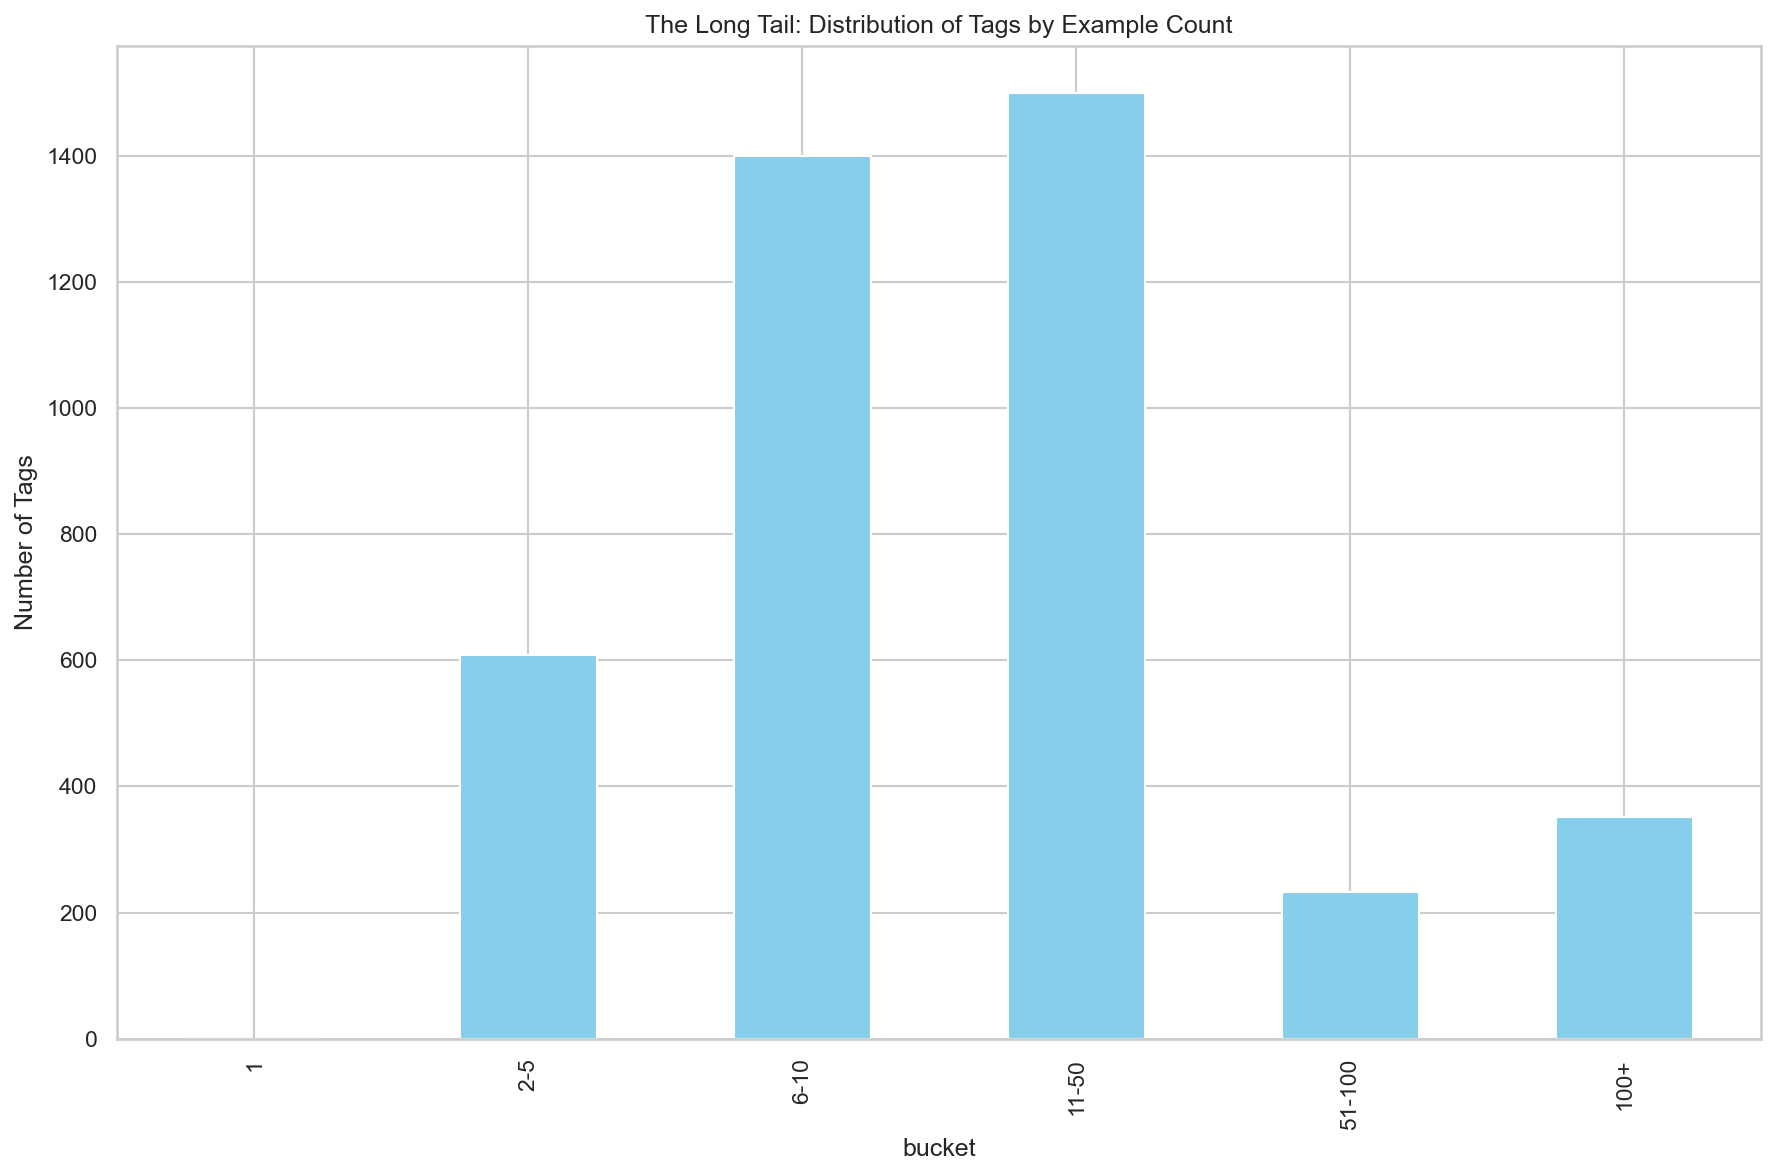
\includegraphics[width=0.9\linewidth]{graphs/final_report/09_tag_long_tail.png}
		\caption{Long-tail distribution of tags by example count. Over 3,000 tags have only a single training example, driving the Micro/Macro-F1 gap.}
		\label{fig:long_tail}
	\end{figure}
	
	\textbf{Ranking metrics.} Despite a modest strict Micro-F1, ranking metrics reveal substantially higher practical utility (Fig.~\ref{fig:hit_rate_k}). Hit Rate@5 of \HitRateFive{} and mAP of \MAPScore{} confirm that correct tags rank well above incorrect ones, supporting deployment as a tag recommender rather than an autonomous classifier.
	
	\textbf{Per-frequency analysis.} F1 drops steeply with training frequency (Fig.~\ref{fig:f1_bucket}, Table~\ref{tab:bucket_f1}): tags with 100+ examples achieve \BucketHead{}, mid-frequency tags (10--100) achieve \BucketMid{}, and tail tags (5--10) drop to \BucketTail{}. Tags with fewer than 5 examples achieve near-zero F1. This long-tail degradation is the primary driver of Macro-F1 depression and the main target for future improvement.
	
	\begin{table}[htbp]
		\centering
		\caption{Per-tag F1 by frequency bucket and tag vocabulary coverage.}
		\label{tab:bucket_f1}
		\begin{tabular}{@{}lrc@{}}
			\toprule
			\textbf{Frequency bucket} & \textbf{Avg.\ F1} & \textbf{Tags with F1$>$0} \\
			\midrule
			Head (100+ examples) & \BucketHead{} & --- \\
			Mid (10--100) & \BucketMid{} & --- \\
			Tail (5--10) & \BucketTail{} & --- \\
			Rare (1--5) & \BucketRare{} & --- \\
			\midrule
			\multicolumn{3}{@{}l}{\textit{Tag coverage thresholds}} \\
			\midrule
			Tags with F1 $>$ 0.5 & \multicolumn{2}{c}{\CovFiveZero{} of \NumTags{}} \\
			Tags with F1 $>$ 0.3 & \multicolumn{2}{c}{\CovThreeZero{} of \NumTags{}} \\
			Tags with F1 $>$ 0.1 & \multicolumn{2}{c}{\CovOneZero{} of \NumTags{}} \\
			Tags with F1 $>$ 0.0 & \multicolumn{2}{c}{\CovAny{} of \NumTags{}} \\
			\bottomrule
		\end{tabular}
	\end{table}
	
	\textbf{Label cardinality mismatch.} The model predicts an average of \PredCardinality{} tags per passage versus a ground-truth average of \GTCardinality{} (ratio \CardinalityRatio{}). This under-prediction is expected: the ground-truth cardinality is inflated by label inheritance (every chunk receives \emph{all} parent tags), while the model assigns only tags relevant to each chunk's content. A ratio of $\sim$0.5 suggests the model performs implicit label denoising. Fig.~\ref{fig:noise_heatmap} confirms this: cosine similarity between chunk embeddings and inherited tag names varies dramatically across chunks, showing that most tag-chunk pairs are semantically mismatched.
	
	\begin{figure}[htbp]
		\centering
		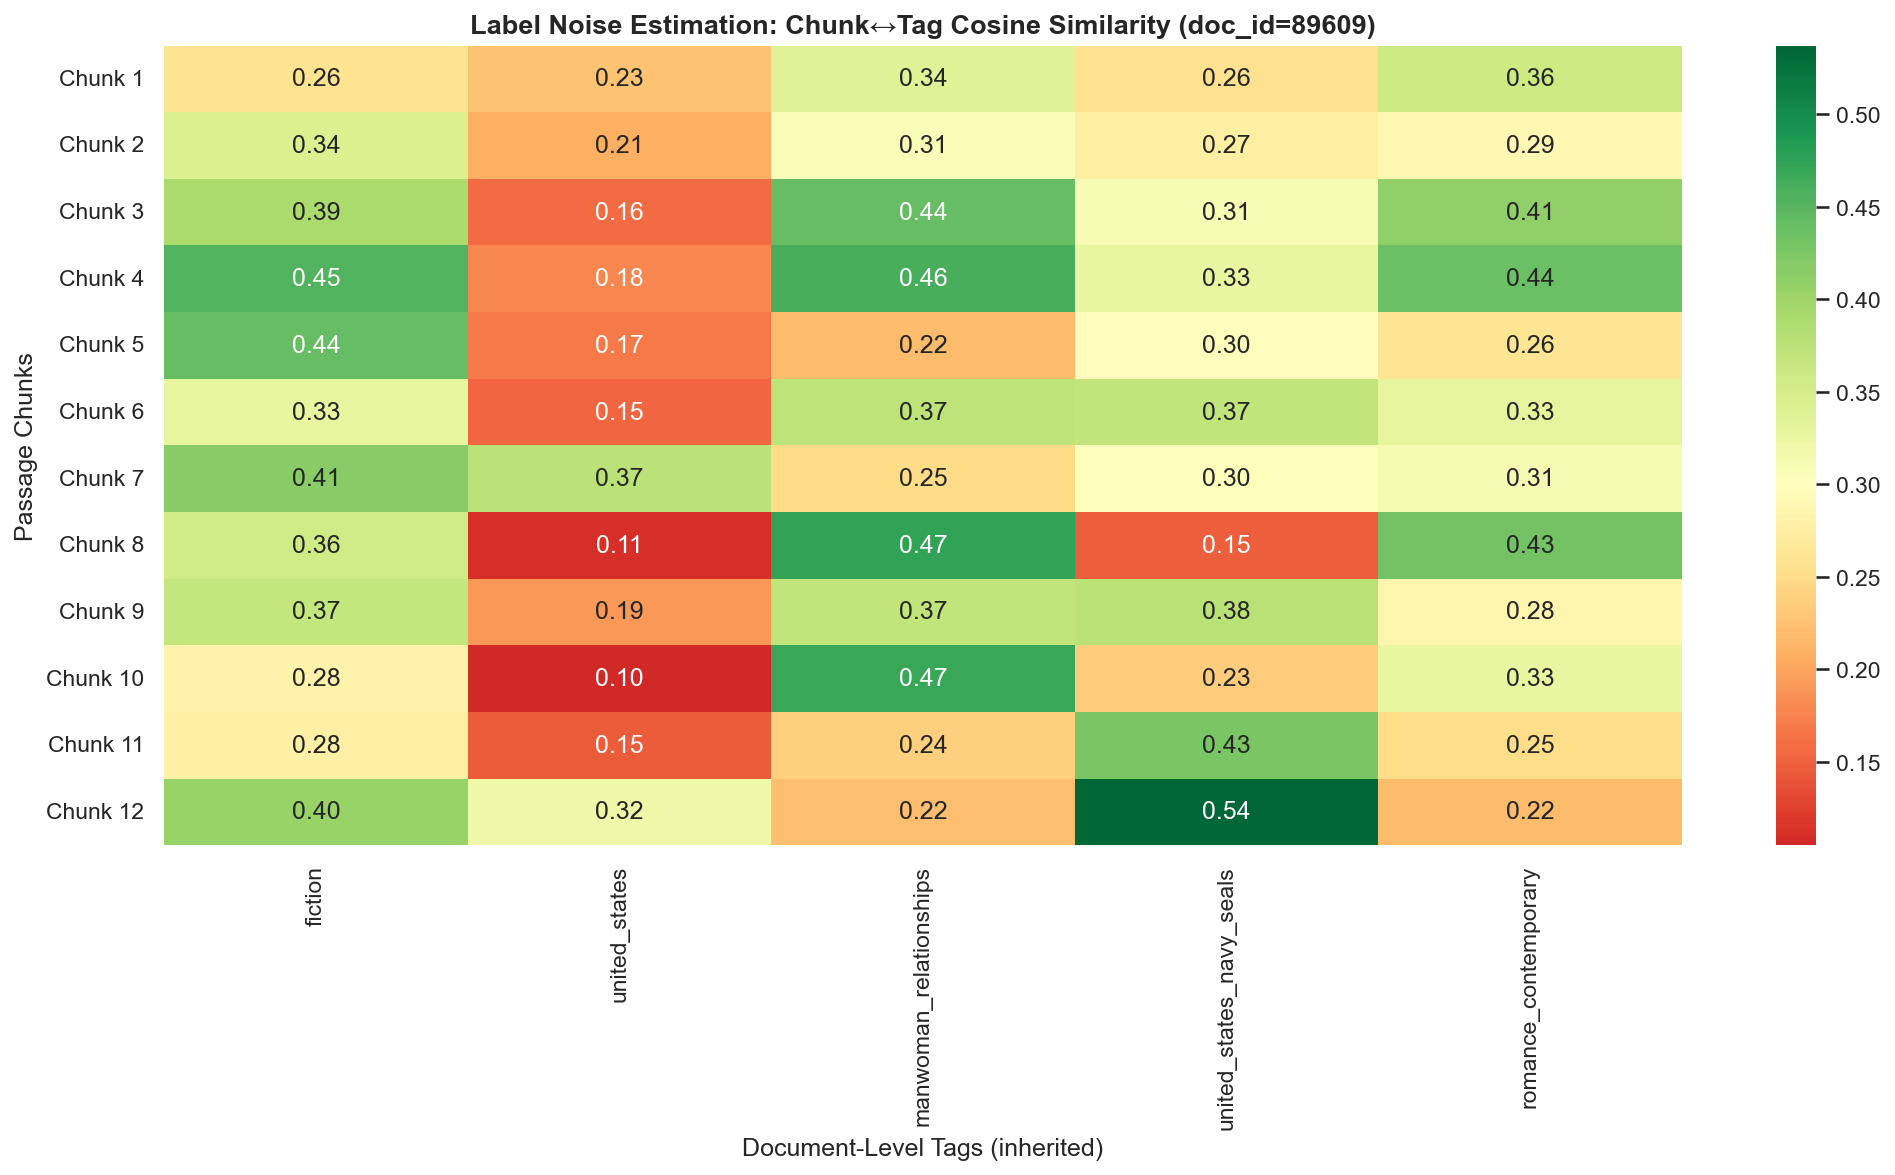
\includegraphics[width=\linewidth]{graphs/final_report_v2/29_label_noise_heatmap.png}
		\caption{Label noise visualization for a sample document. Each cell shows the cosine similarity between a passage chunk's embedding and an inherited tag name, confirming that document-level tags are a poor proxy for passage-level content.}
		\label{fig:noise_heatmap}
	\end{figure}
	
	The precision-recall curve (Fig.~\ref{fig:pr_curve}) shows well-calibrated outputs (precision 0.81 at $t{=}0.50$, recall 0.55 at $t{=}0.15$).
	
	\subsection{\texttt{pos\_weight} Failure and Recovery}
	\label{sec:posweight}
	Training with \texttt{pos\_weight} set to the negative/positive ratio per tag (up to $\PosWeightMax{}\times$ for rare tags) pinned Micro-F1 at \PosWeightMicroF{} across all epochs. The model collapsed to predicting the majority class, and the amplified positive-class gradient magnified contributions from mislabeled chunks, reinforcing the collapse.
	
	Removing \texttt{pos\_weight} and using standard \texttt{BCEWithLogitsLoss} immediately restored training dynamics. By epoch 4, Micro-F1 reached \NoPosWeightEpochFour{} and continued climbing; training loss fell from \EPUBLossStart{} to \EPUBLossFinal{}. The final model achieves Micro-F1 of \MicroF{} at optimal threshold \EPUBOptThreshold{} (Fig.~\ref{fig:threshold_sweep}), a gain of $+$\PosWeightDelta{} points over the weighted baseline.
	
	
	
	\begin{figure}[htbp]
		\centering
		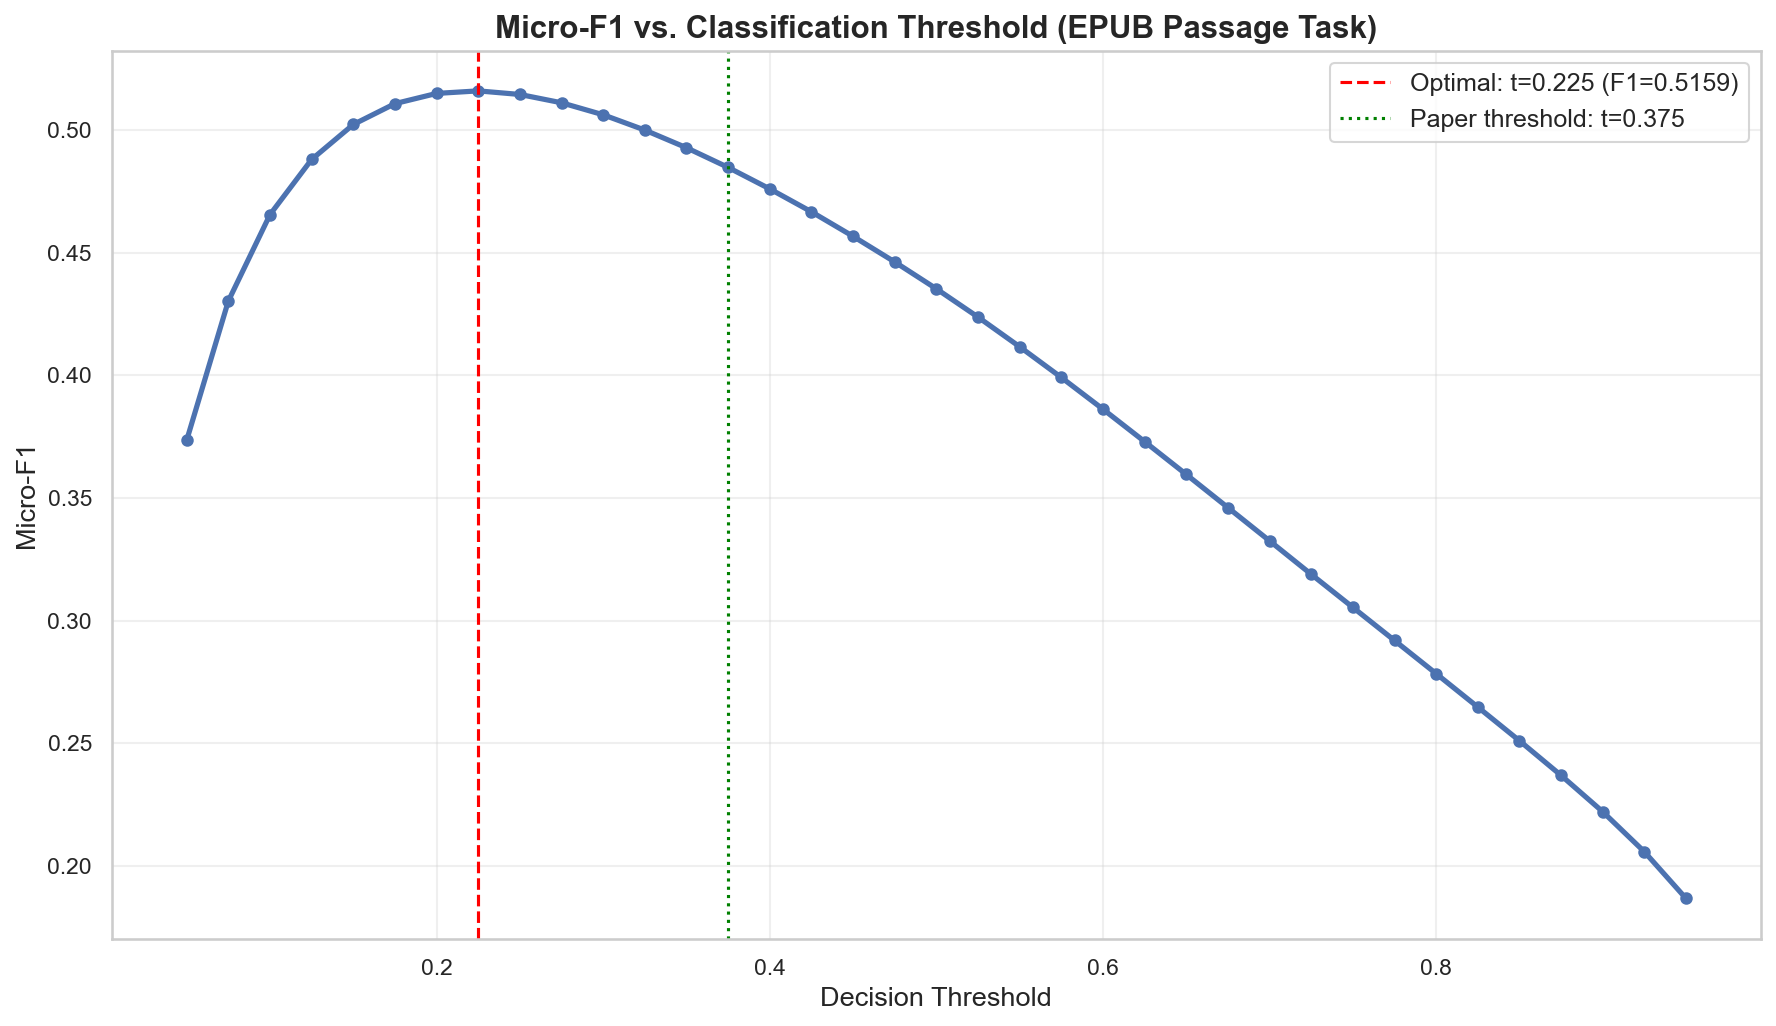
\includegraphics[width=\linewidth]{graphs/final_report_v2/24_threshold_sweep_f1.png}
		\caption{Micro-F1 as a function of decision threshold. The optimal threshold of \EPUBOptThreshold{} yields Micro-F1 of \EPUBOptThresholdF{}, reflecting the noise characteristics of document-inherited labels.}
		\label{fig:threshold_sweep}
	\end{figure}
	
	
	
%	\begin{figure}[htbp]
%		\centering
%		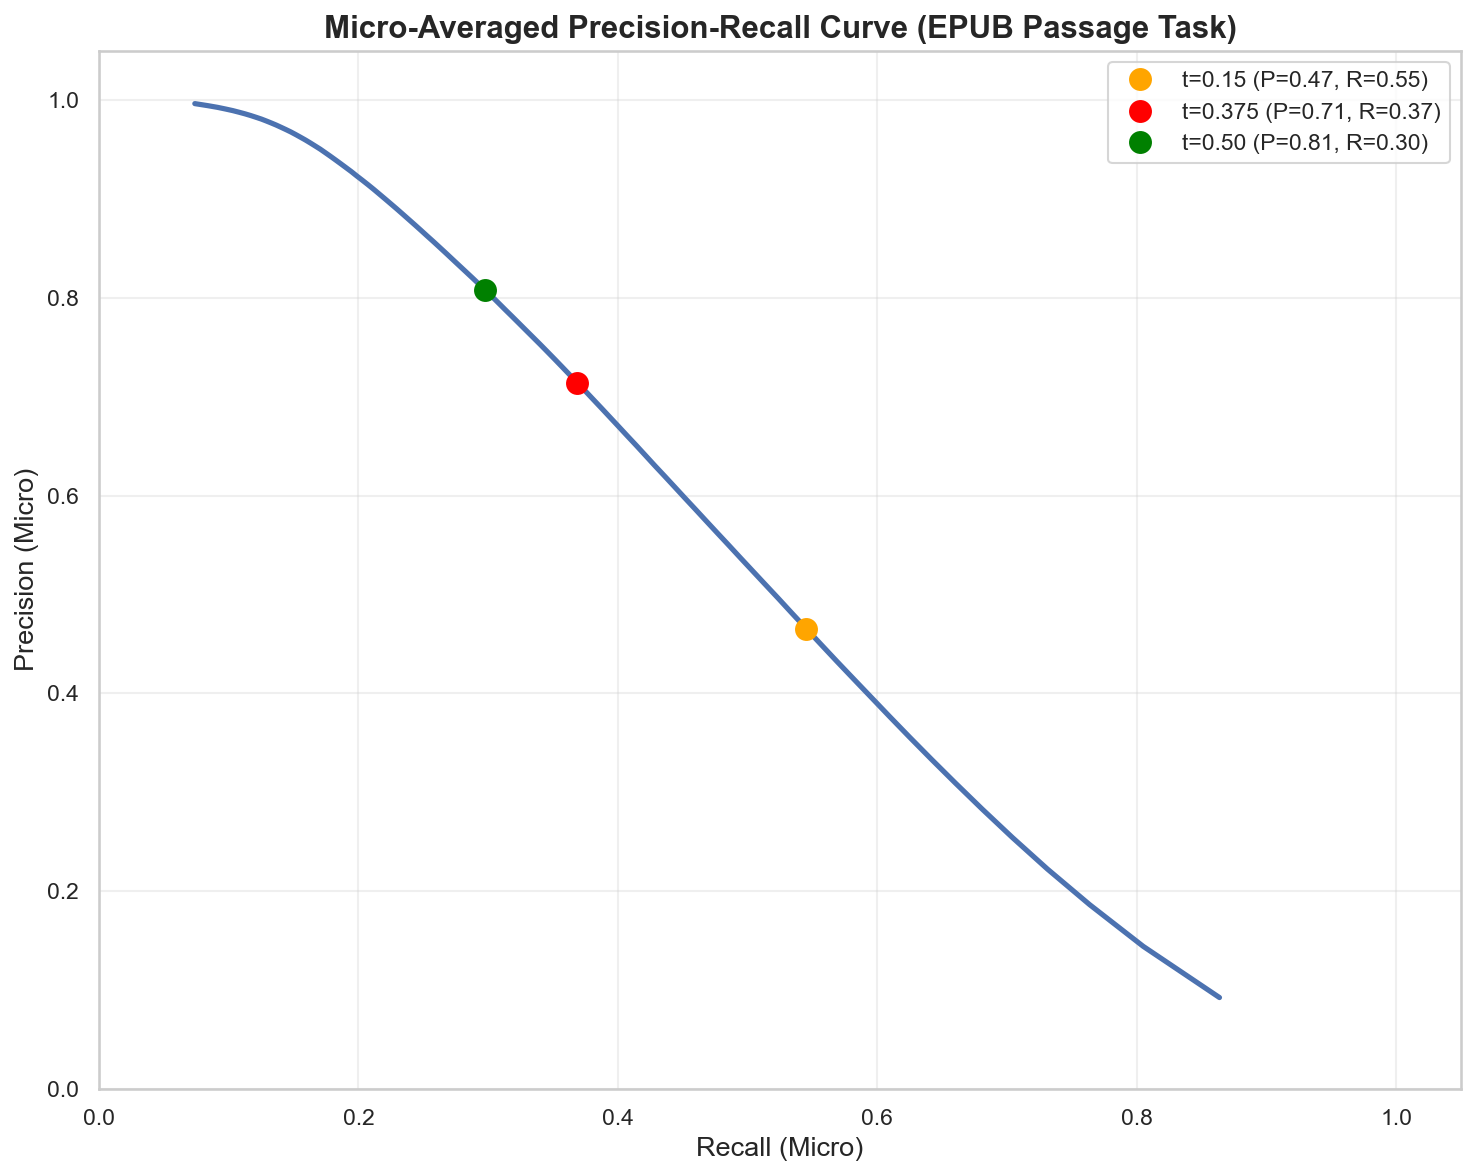
\includegraphics[width=\linewidth]{graphs/final_report_v2/30_precision_recall_curve.png}
%		\caption{Micro-averaged precision-recall curve. Three operating points are annotated: $t{=}0.15$ (high recall, P=0.47/R=0.55), $t{=}0.375$ (balanced, P=0.71/R=0.37), and $t{=}0.50$ (high precision, P=0.81/R=0.30). The smooth curve confirms well-calibrated probability outputs despite the noisy training labels.}
%		\label{fig:pr_curve}
%	\end{figure}
	
	
	
	\begin{figure}[htbp]
		\centering
		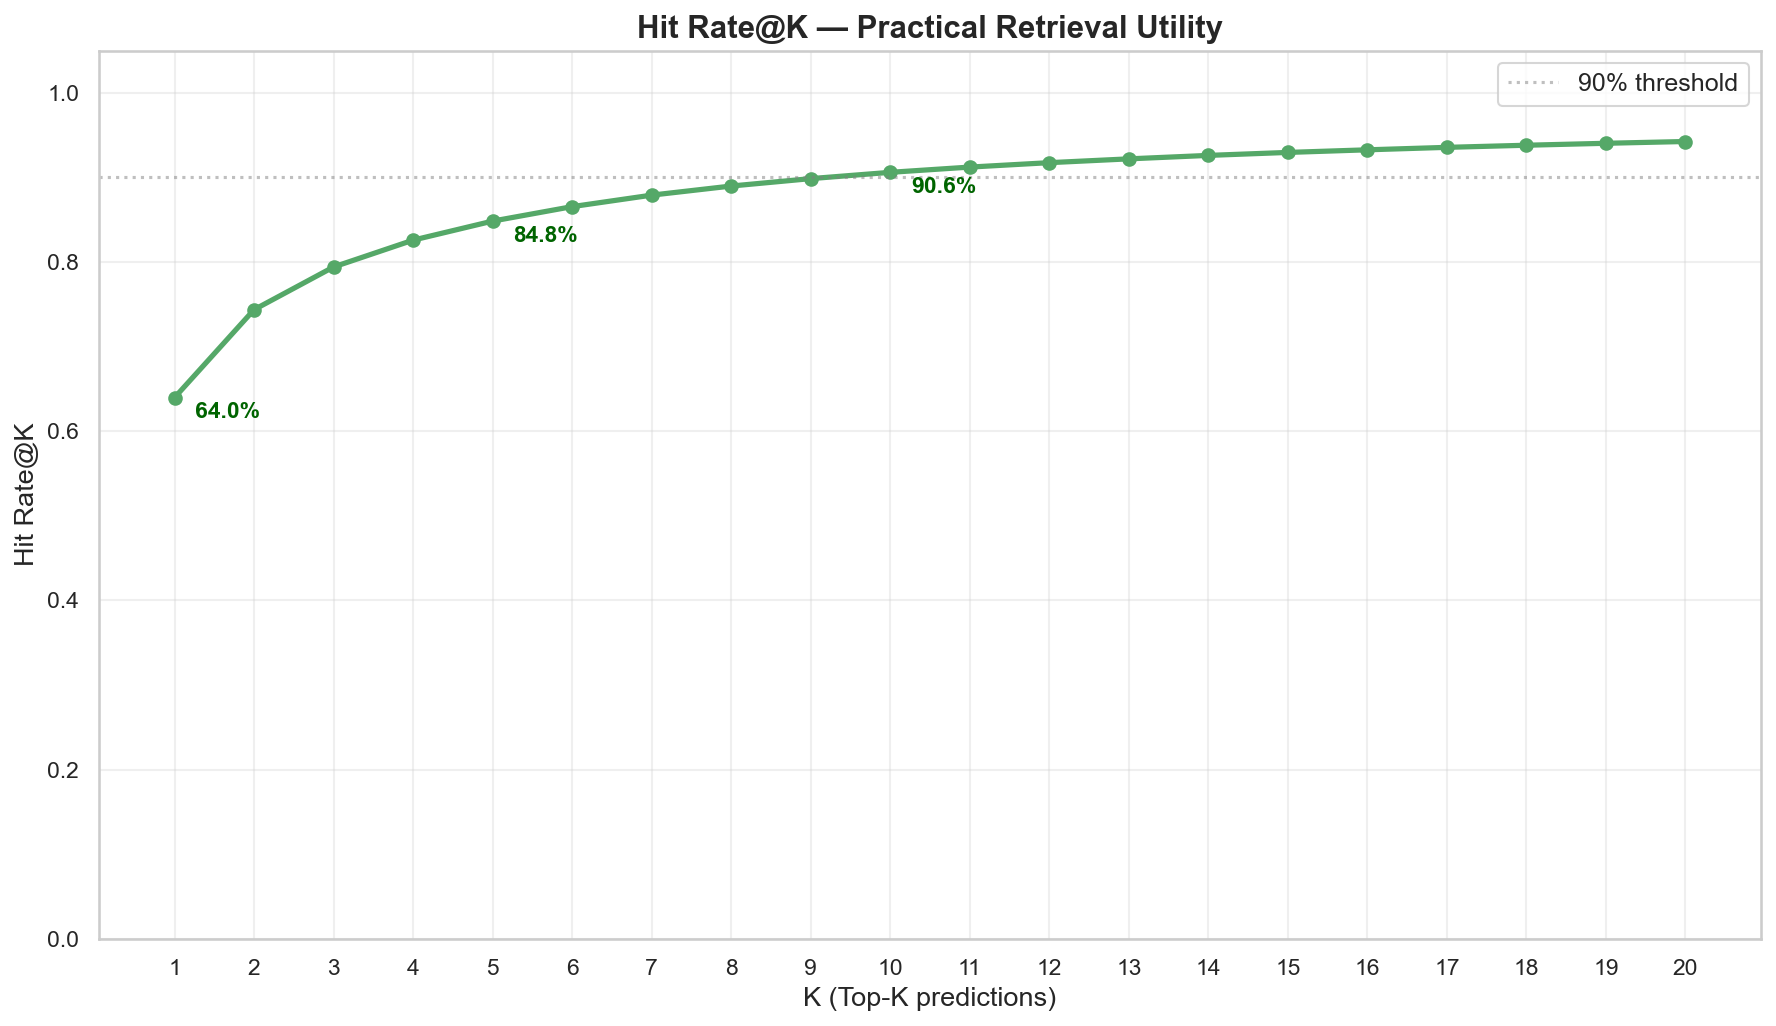
\includegraphics[width=\linewidth]{graphs/final_report_v2/25_hit_rate_at_k.png}
		\caption{Hit Rate@$K$ for the combined corpus. At $K{=}5$, 84.8\% of passages have at least one correct tag in their top-5 predictions, rising to 90.6\% at $K{=}10$, demonstrating practical utility as a tag recommender despite the modest strict F1.}
		\label{fig:hit_rate_k}
	\end{figure}
	
	
	
	
	\begin{figure}[htbp]
		\centering
		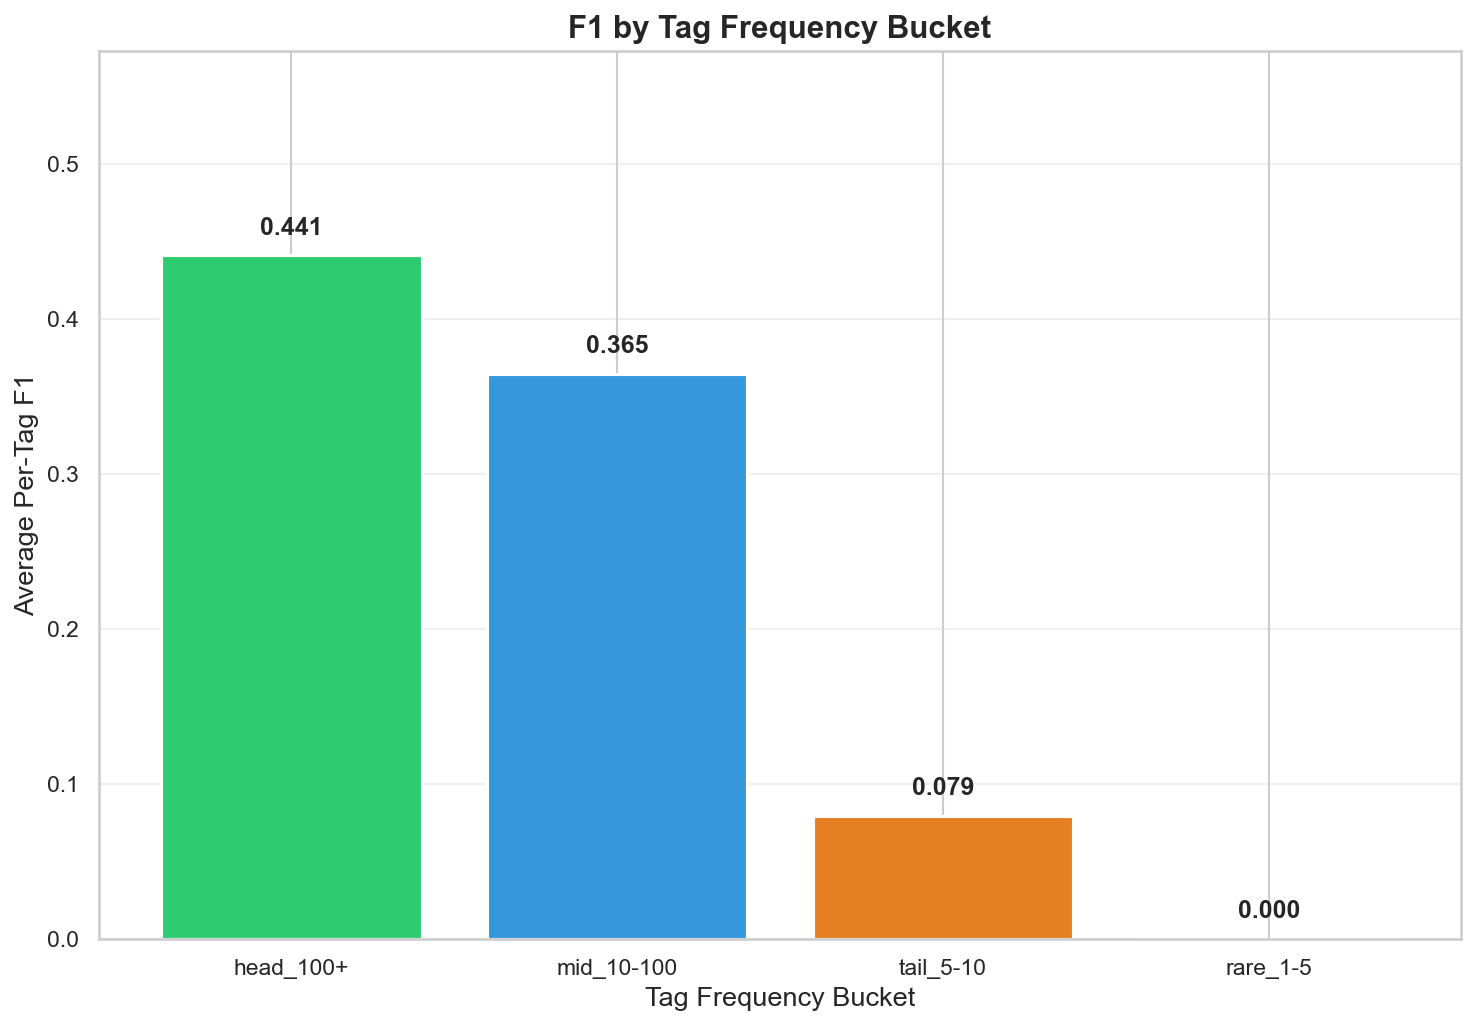
\includegraphics[width=\linewidth]{graphs/final_report_v2/27_f1_by_frequency_bucket.png}
		\caption{Average per-tag F1 by frequency bucket. The steep drop from head (\BucketHead{}) to tail (\BucketTail{}) confirms that improving tail-tag performance is the primary avenue for future gains.}
		\label{fig:f1_bucket}
	\end{figure}
	
	
	\subsection{Training Dynamics}
	The training dynamics reveal a critical interaction between loss function design and label noise (Fig.~\ref{fig:posweight_f1}). With \texttt{pos\_weight} enabled (weights up to $\PosWeightMax{}\times$), Micro-F1 remained flat at $\sim$\PosWeightMicroF{} for the entire run, indistinguishable from the all-zeros baseline. The loss curves (Fig.~\ref{fig:posweight_loss}) reveal a critical diagnostic: both configurations show decreasing loss, but only the unweighted run translates this into improving F1. The \texttt{pos\_weight} run's loss decreases because the model learns to predict all-zeros more confidently, a deceptive convergence undetectable by monitoring loss alone. Removing \texttt{pos\_weight} immediately normalized training: Micro-F1 reached \NoPosWeightEpochFour{} by epoch 4 and continued climbing, while loss fell from \EPUBLossStart{} to \EPUBLossFinal{}. This before/after contrast (same architecture, same data, different loss configuration) isolates the failure precisely: \texttt{pos\_weight} amplifies the gradient from every positive label, and when a substantial fraction of positives are incorrect, this amplification overwhelms the genuine learning signal. On the ArXiv-only subset with clean labels, the same architecture converges smoothly to Micro-F1 of \ArXivMicroF{} with a narrow train-validation gap, confirming that the architecture is not the bottleneck.
	
	
	
	\begin{figure}[htbp]
		\centering
		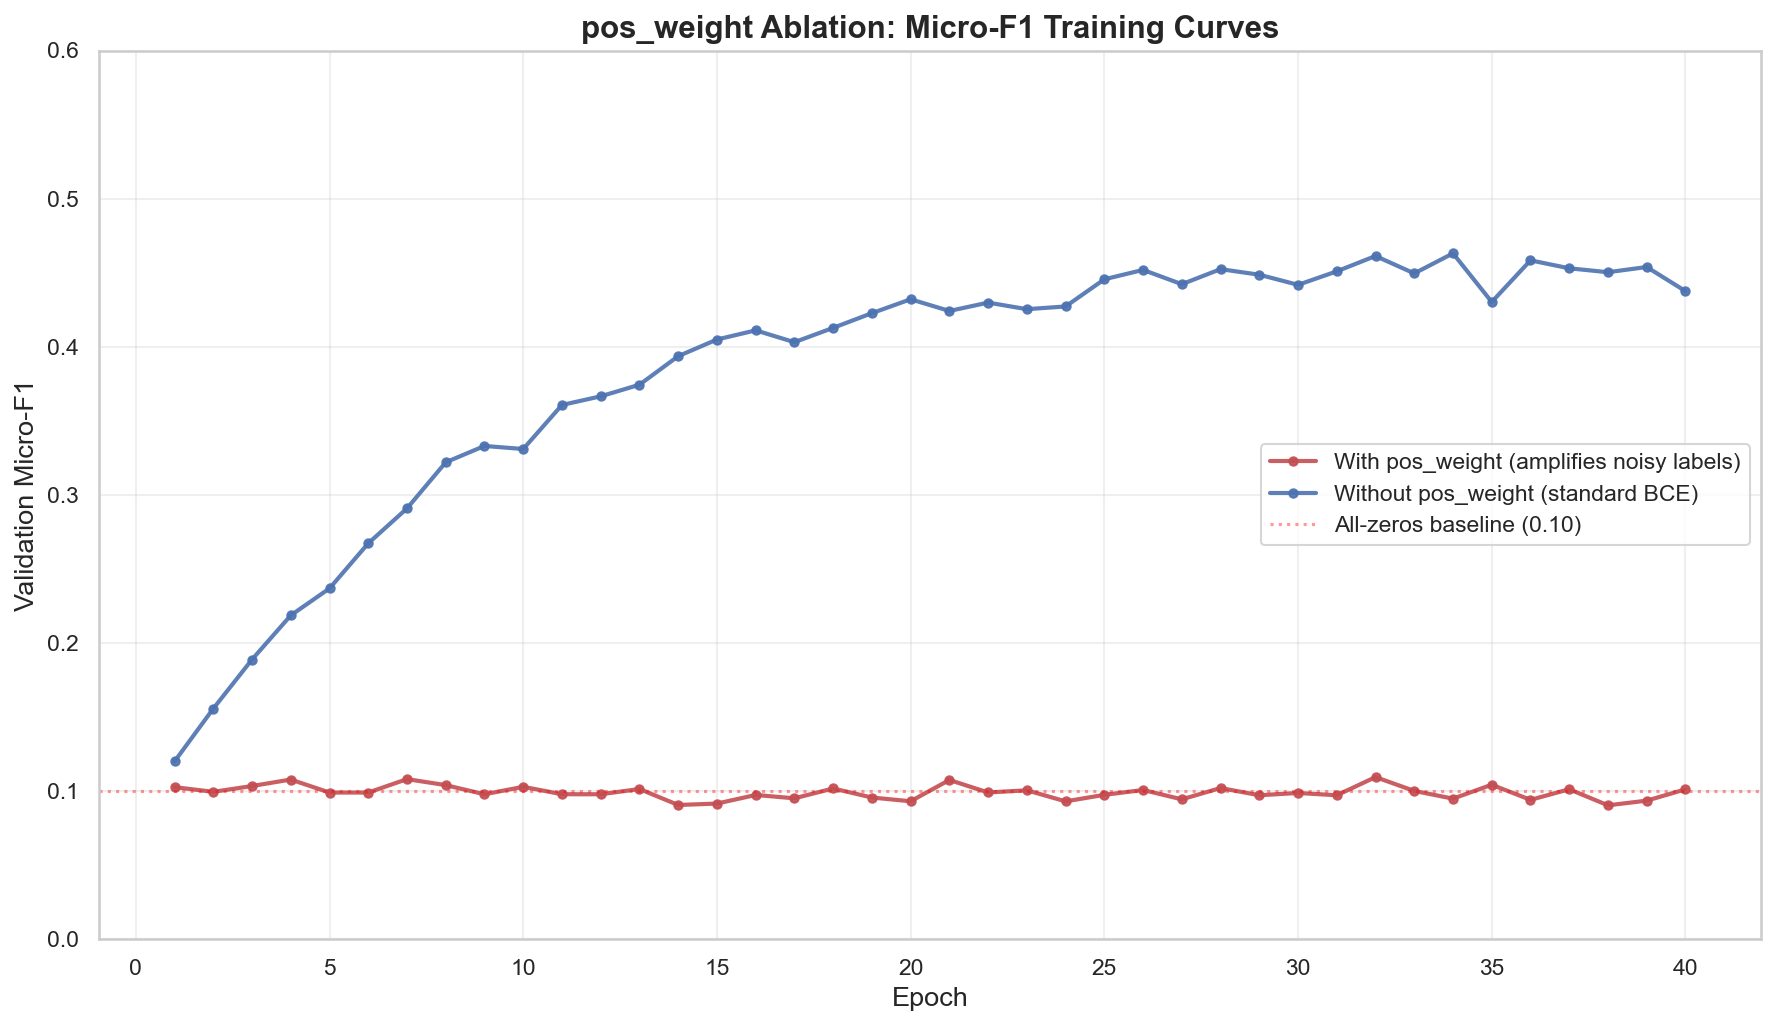
\includegraphics[width=\linewidth]{graphs/final_report_v2/22_posweight_vs_standard_f1.png}
		\caption{\texttt{pos\_weight} ablation: Micro-F1 training curves. With \texttt{pos\_weight} (red), F1 remains pinned at the all-zeros baseline ($\sim$\PosWeightMicroF{}) for all 40 epochs. Without \texttt{pos\_weight} (blue), F1 climbs steadily to \MicroF{}, confirming that the architecture learns effectively once the loss function stops amplifying noisy labels.}
		\label{fig:posweight_f1}
	\end{figure}
	
	
	
	\begin{figure}[htbp]
		\centering
		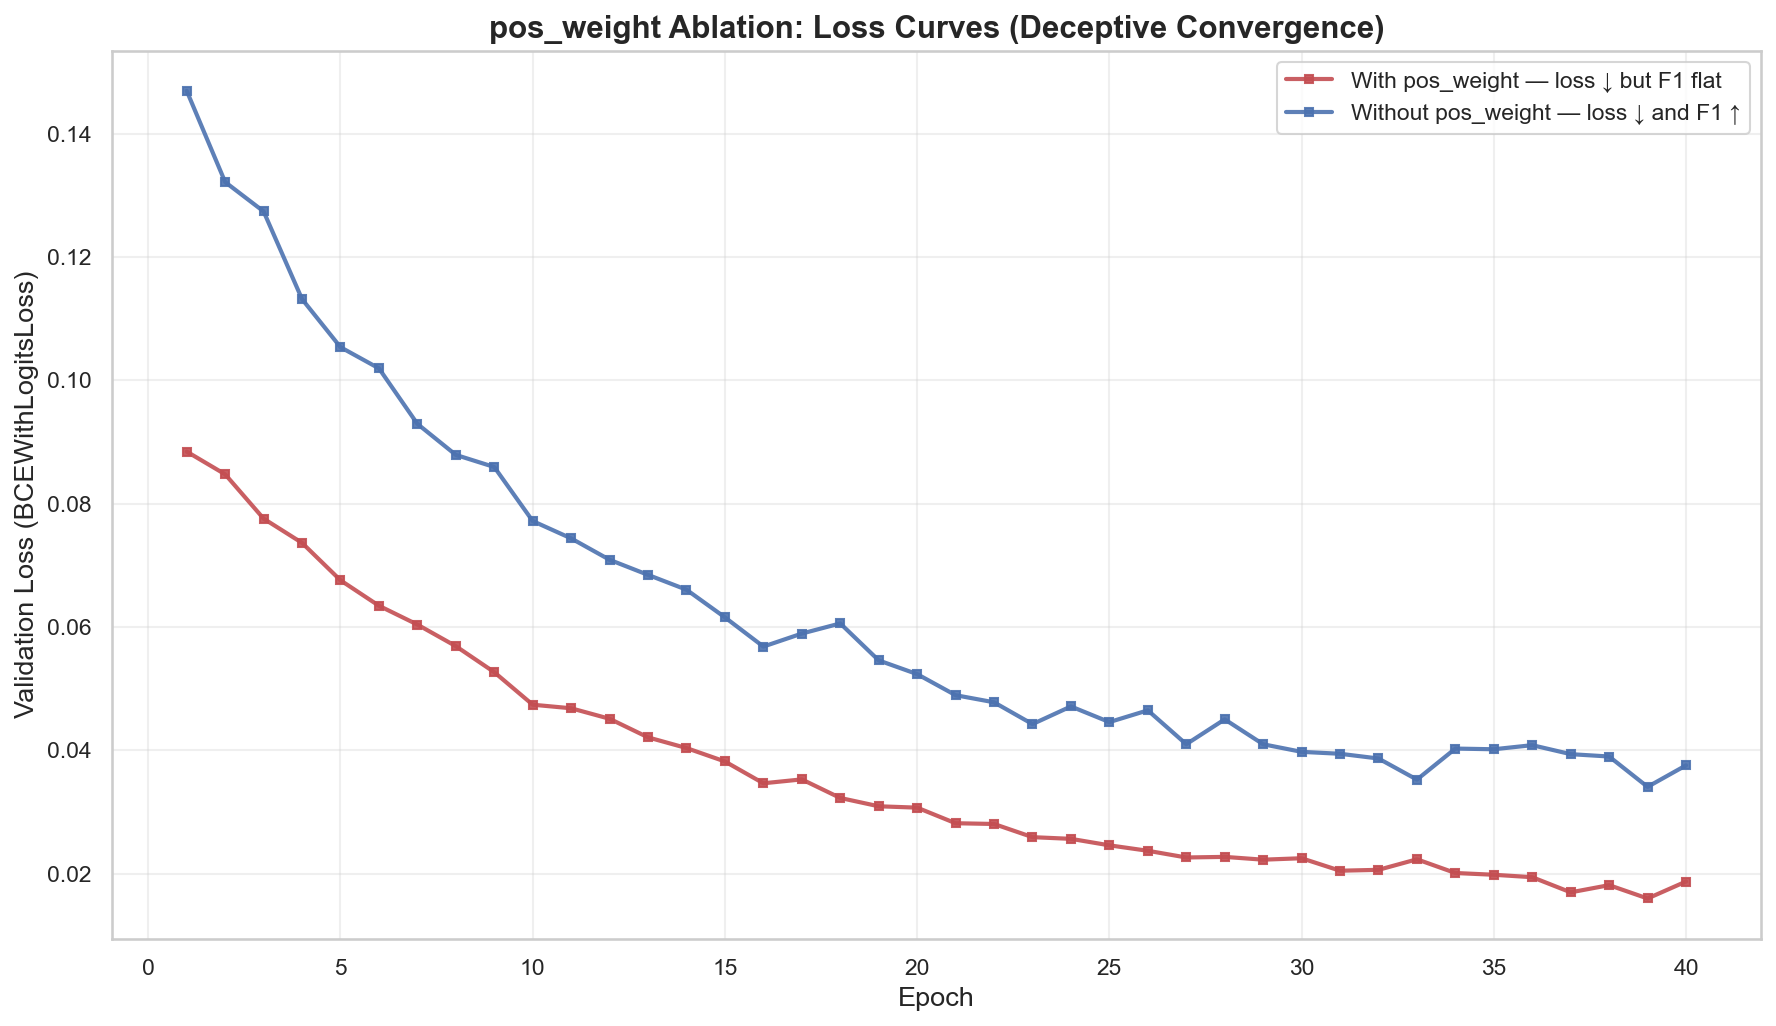
\includegraphics[width=\linewidth]{graphs/final_report_v2/23_posweight_vs_standard_loss.png}
		\caption{\texttt{pos\_weight} ablation: loss curves (deceptive convergence). Both configurations show decreasing loss, but the \texttt{pos\_weight} run (red) achieves lower absolute loss by learning to predict all-zeros more confidently, a failure mode invisible to loss monitoring alone. Only the unweighted run (blue) translates decreasing loss into improving F1 (cf.\ Fig.~\ref{fig:posweight_f1}).}
		\label{fig:posweight_loss}
	\end{figure}
	
	
	\subsection{Ablation Study}
	To quantify the contribution of each architectural decision, I compared the full pipeline against four ablation variants (Table \ref{tab:ablation}).
	
	\begin{table}[htbp]
		\centering
		\caption{Ablation study. Top rows: ArXiv-only subset with clean labels. Bottom rows: combined corpus with document-inherited labels. OvR = One-vs-Rest Logistic Regression; MLP = Multi-Layer Perceptron; Ens = weighted ensemble. ``FT'' = contrastive fine-tuned encoder.}
		\label{tab:ablation}
		\begin{tabular}{@{}lccc@{}}
			\toprule
			\textbf{Configuration} & \textbf{Micro-F1} & \textbf{Macro-F1} & \textbf{Threshold} \\
			\midrule
			\multicolumn{4}{@{}l}{\textit{ArXiv-only (clean document-level labels)}} \\
			FT Encoder + MLP & \textbf{\AblMLPOptMicro{}} & \textbf{\AblMLPOptMacro{}} & per-tag opt. \\
			FT Encoder + OvR & \AblOvROptMicro{} & \AblOvROptMacro{} & per-tag opt. \\
			FT Encoder + MLP & \AblMLPGlobalMicro{} & \AblMLPGlobalMacro{} & global \GlobalThreshold{} \\
			FT Encoder + OvR & \AblOvRGlobalMicro{} & \AblOvRGlobalMacro{} & global 0.50 \\
			Ensemble (MLP + OvR) & \AblEnsOptMicro{} & \AblEnsOptMacro{} & per-tag opt. \\
			\midrule
			\multicolumn{4}{@{}l}{\textit{Combined corpus (document-inherited passage labels)}} \\
			FT Encoder + MLP + \texttt{pw} & $\sim$\PosWeightMicroF{} & --- & per-tag opt. \\
			FT Encoder + MLP $-$ \texttt{pw} & \MicroF{} & \MacroF{} & per-tag opt. \\
			\bottomrule
		\end{tabular}
	\end{table}
	
	The results demonstrate two clear findings. First, the MLP head consistently outperforms the OvR logistic regression baseline by 3--4 points in Micro-F1, confirming that the mapping from the \EncoderDim{}-dimensional embedding to \NumTagsAblation{} labels benefits from non-linear capacity. Second, per-tag threshold optimization on the validation set yields a 3-point improvement over the fixed global threshold, particularly for medium-frequency tags where the optimal decision boundary deviates substantially from 0.5.
	
	\textbf{Loss function ablation.} The final two rows of Table~\ref{tab:ablation} show the primary combined-corpus evaluation, isolating \texttt{pos\_weight} as the sole variable. With \texttt{pos\_weight} enabled (values up to $\PosWeightMax{}\times$ for rare tags), Micro-F1 collapses to $\sim$\PosWeightMicroF{}. Removing it while holding all other hyperparameters constant recovers performance to \MicroF{}, a \PosWeightDelta{}-point improvement attributable entirely to the loss configuration. The upper rows show that on the ArXiv-only subset with clean labels, the same MLP architecture with per-tag threshold optimization reaches \ArXivMicroF{}. The updated ablation (Fig.~\ref{fig:ablation_updated}) visualizes all configurations.
	
	
	\begin{figure}[htbp]
		\centering
		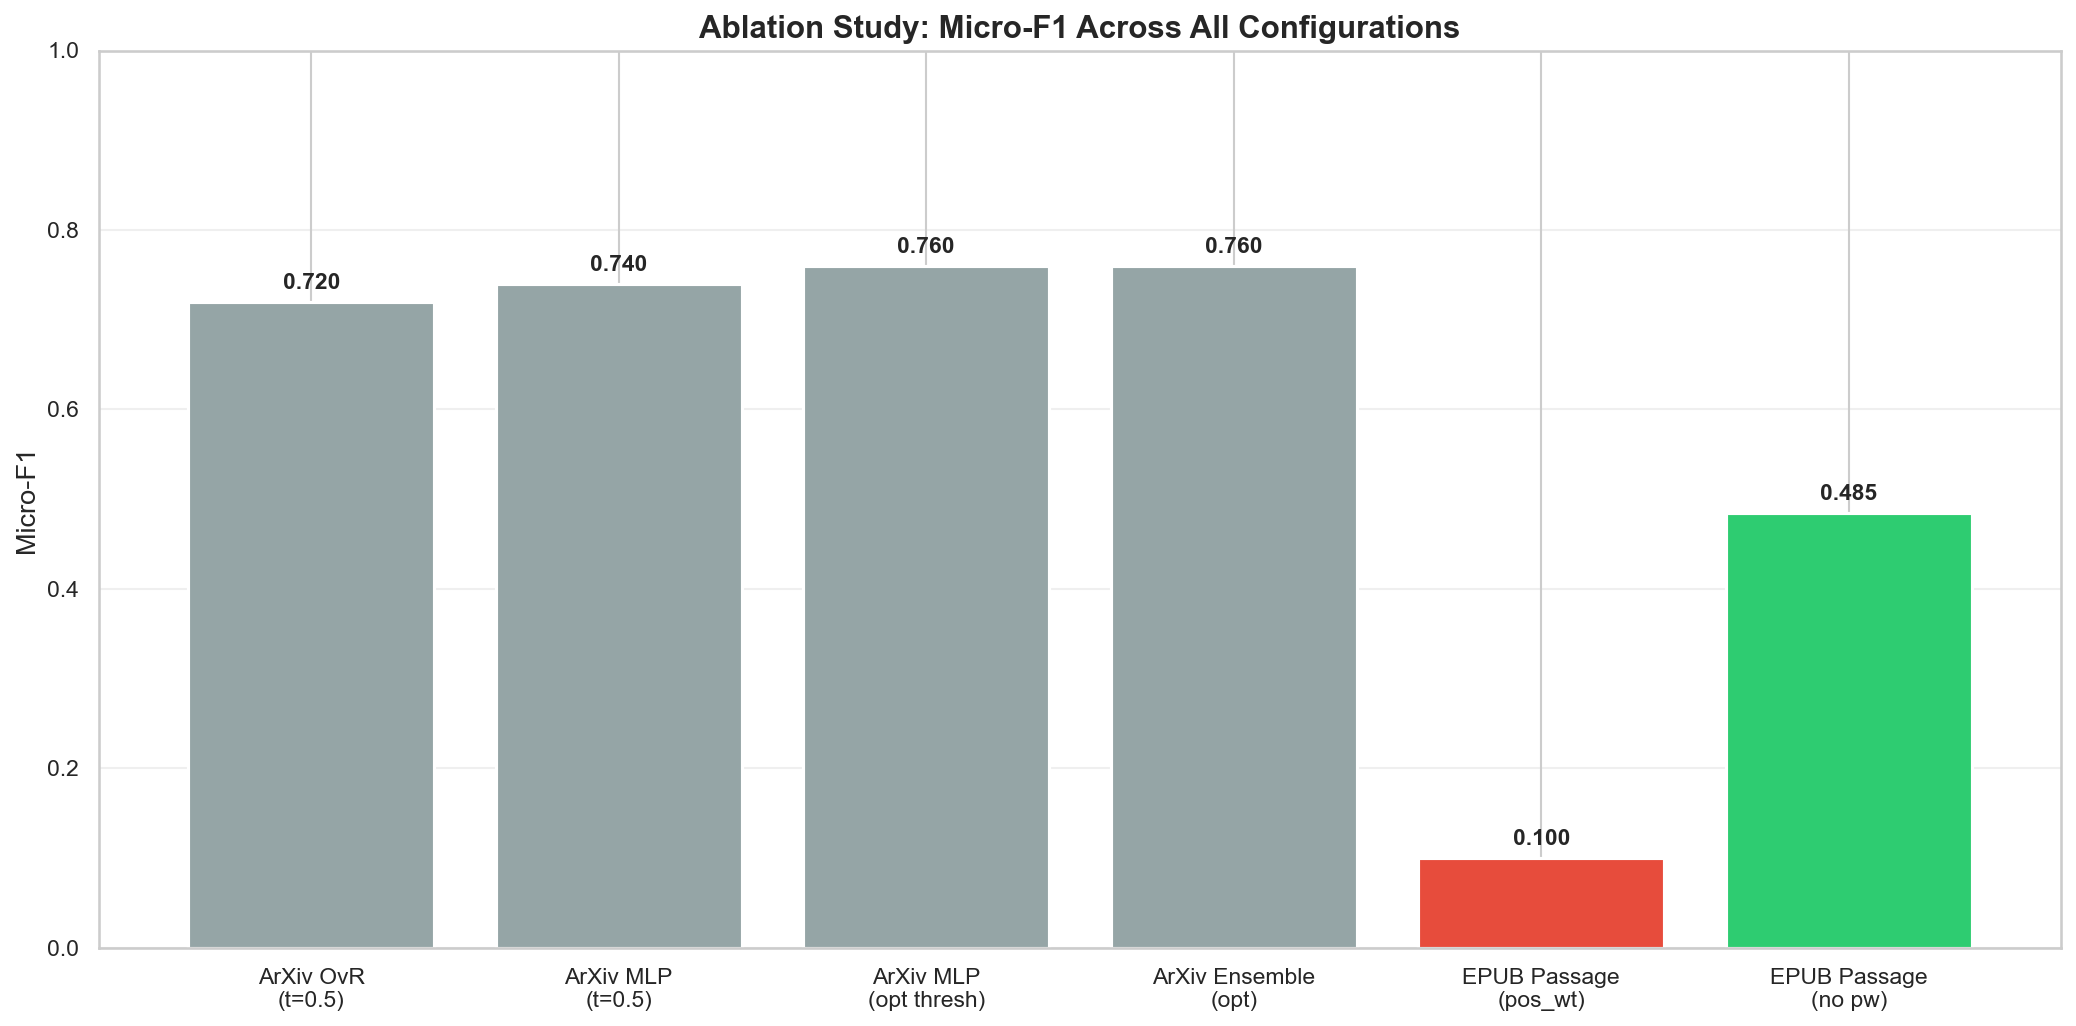
\includegraphics[width=\linewidth]{graphs/final_report_v2/28_ablation_bar_chart.png}
		\caption{Extended ablation study. The upper bars show ArXiv-only configurations; the rightmost pair shows the combined corpus with and without \texttt{pos\_weight}. The \PosWeightDelta{}-point gap isolates the effect of \texttt{pos\_weight} under noisy inherited labels.}
		\label{fig:ablation_updated}
	\end{figure}
	
	
	\subsection{Per-Tag Confidence Analysis}
	When analyzing prediction confidence by tag (Fig. \ref{fig:high_conf}), I observed a significant disparity between established core sciences and niche, interdisciplinary domains. The model exhibits its highest confidence in fields such as astrophysics, statistics, and mathematics, which possess rigid, highly distinct technical vocabularies that the contrastive learning stage mapped efficiently. Conversely, the model exhibited higher false-positive rates and lower overall confidence in interdisciplinary areas, such as quantitative biology or computational finance, where the vocabulary overlaps heavily with neighboring disciplines.
	
	\begin{figure}[htbp]
		\centering
		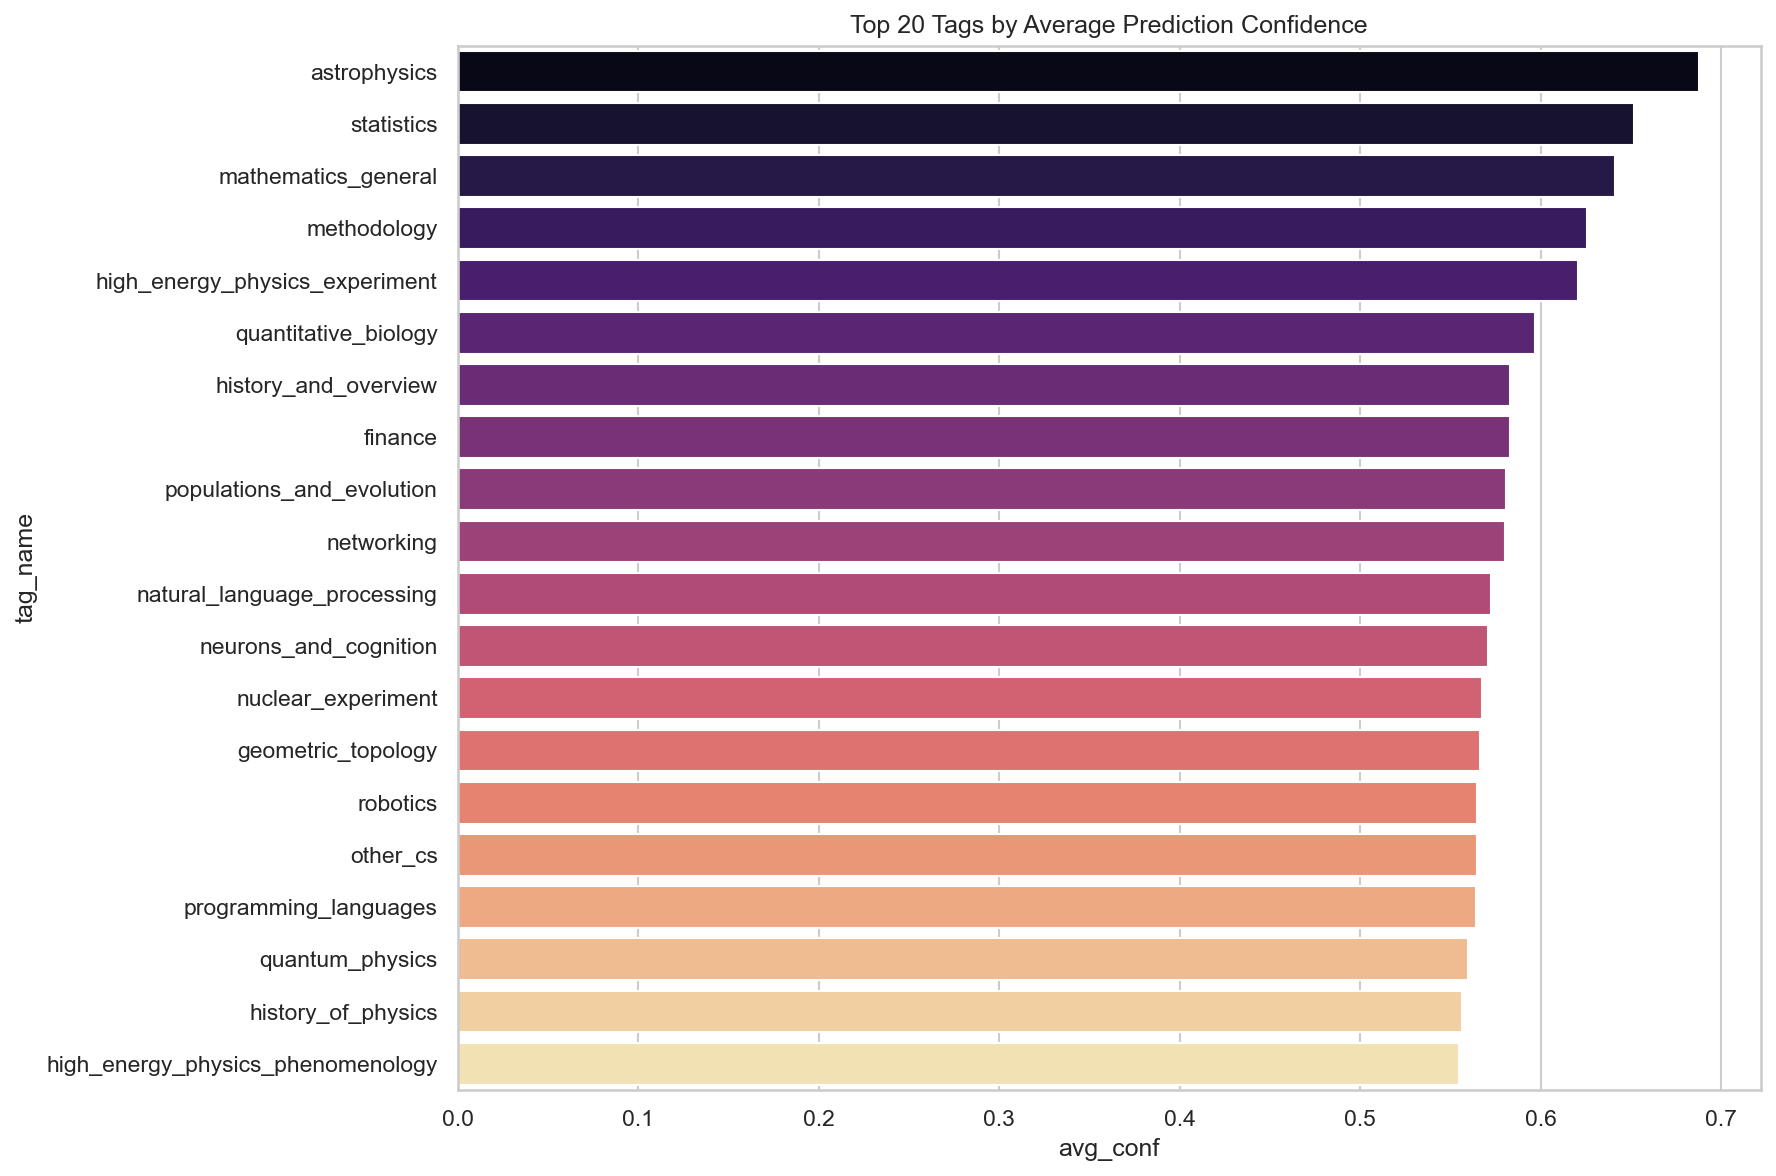
\includegraphics[width=0.8\linewidth]{graphs/final_report/08_highest_confidence_tags.png}
		\caption{Tags with highest average prediction confidence. Core sciences show the strongest model certainty.}
		\label{fig:high_conf}
	\end{figure}
	
	This variance in predictive confidence confirms that the \texttt{all-MiniLM-L6-v2} encoder relies heavily on lexical density. When the text lacks domain-exclusive terminology, the embedding falls near the center of the representation space, producing a wider distribution of lower-confidence logits across the MLP output layer.
	
	% NOTE: Figure 26_probability_distribution_by_domain.png was not generated.
	% Uncomment and update path once this chart is available.
	%\begin{figure}[htbp]
	%	\centering
	%	\includegraphics[width=\linewidth]{graphs/final_report/26_probability_distribution_by_domain.png}
	%	\caption{Output logit probability distributions for a core science tag (algebraic geometry) vs.\ an interdisciplinary tag (ML + Finance). The sharper concentration of the core science distribution explains its higher prediction confidence.}
	%	\label{fig:logit_distribution}
	%\end{figure}
	
	\subsection{Threshold Optimization}
	Rather than using a single global threshold, I performed per-tag threshold optimization on the validation set by sweeping 19 threshold values between 0.05 and 0.95 for each of the \NumTags{} tags independently, selecting the value that maximized per-tag F1. For tags with fewer than 10 positive validation examples, I fell back to a global threshold of \GlobalThreshold{}. Fig.\ \ref{fig:threshold_dist} shows the resulting distribution: the majority of tags settle between 0.20 and 0.50, with substantial spread confirming that a single threshold is suboptimal for this label space.
	
	\begin{figure}[htbp]
		\centering
		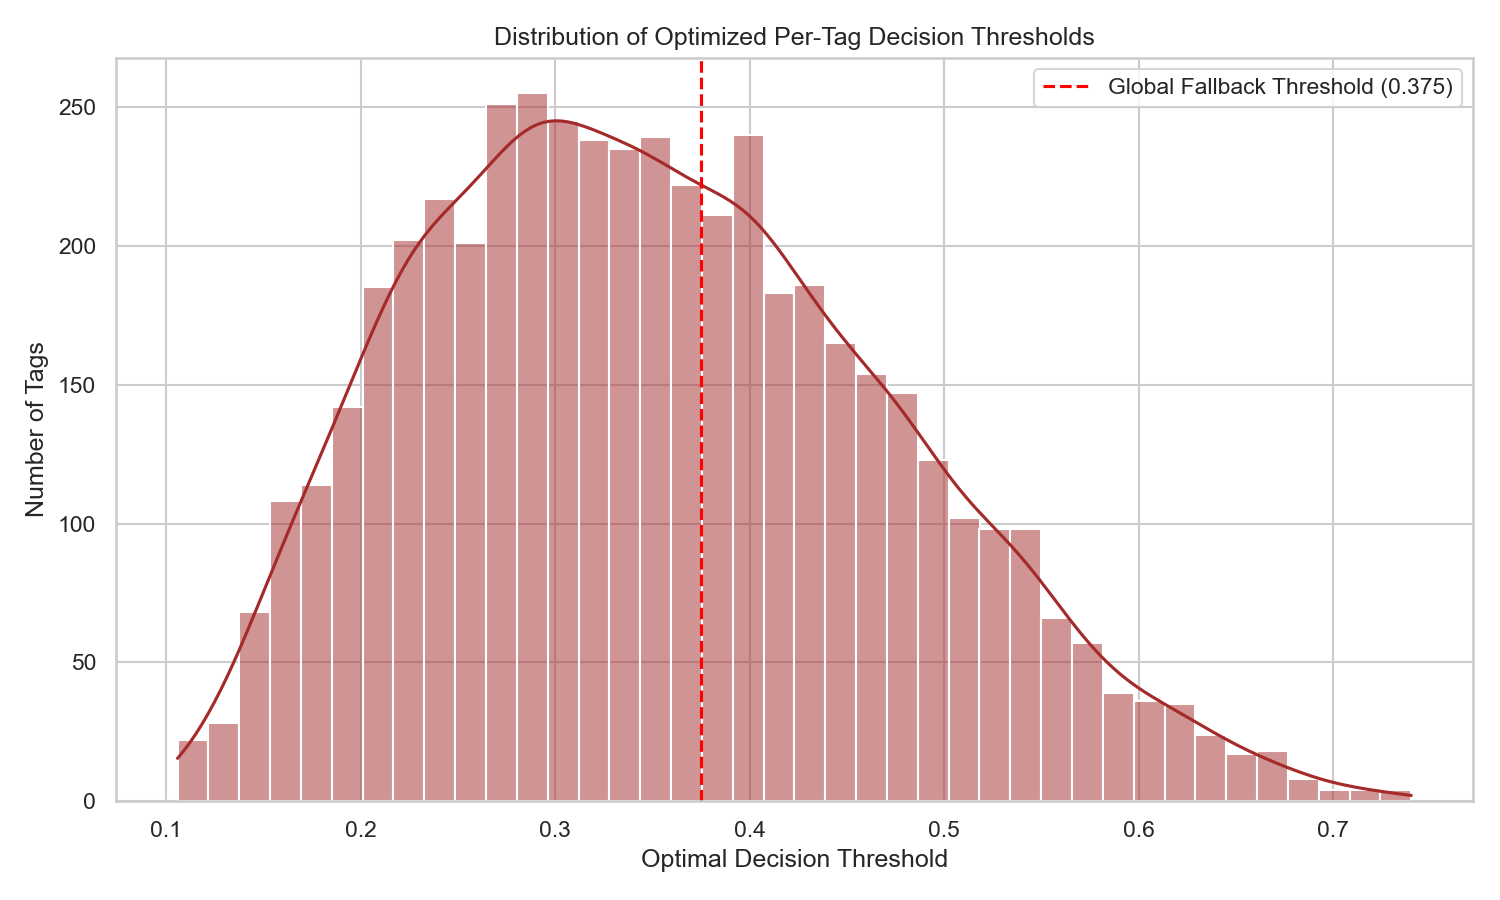
\includegraphics[width=\linewidth]{graphs/final_report/25_per_tag_threshold_distribution.png}
		\caption{Distribution of optimized per-tag decision thresholds across \NumTags{} tags. The global fallback (\GlobalThreshold{}, dashed red) sits near the mode, but individual tags range from 0.10 to 0.70+, justifying per-tag optimization.}
		\label{fig:threshold_dist}
	\end{figure}
	
	
	\section{Discussion and Limitations}
	
	The implementation demonstrates that SetFit is a viable architecture for high-cardinality classification at production scale. However, several limitations merit discussion.
	
	\textbf{1) Long-Tail Label Sparsity:} 
	Over 3,000 of the \NumTags{} tags have only a single training example, fundamentally limiting per-tag recall. The Macro-F1 of \MacroF{} reflects this: the model achieves F1 of \BucketHead{} on head tags (100+ examples) but \BucketRare{} on rare tags (1–5 examples). Future work should explore focal loss, label-aware sampling, or cost-sensitive learning.
	
	\textbf{2) Out-of-Vocabulary (OOV) Terms:} 
	Specialized emerging fields suffer from semantic drift when niche compound terms are split into subword tokens that lose domain-specific signal. Longer-context encoders (e.g., Longformer, ModernBERT) could mitigate this.
	
	\textbf{3) Label Source Heterogeneity:} 
	The corpus combines five label sources of varying granularity: ArXiv categories (coarse, structured) and ISBN subjects (fine-grained, noisy). Document-level ArXiv performance (\ArXivMicroF{}) versus full-corpus performance (\MicroF{}) quantifies this difference. Cross-source evaluation would further reveal generalization limits.
	
\textbf{4) Label Granularity Mismatch and Loss Function Sensitivity:} 
Document-level tags assigned to passages introduce systematic noise, since most tags apply globally but not locally. The cardinality ratio of \CardinalityRatio{} (predicted \PredCardinality{} vs.\ ground truth \GTCardinality{} per passage) shows the model implicitly denoises by predicting roughly half the inherited tags. Standard \texttt{BCEWithLogitsLoss} tolerates this noise, but \texttt{pos\_weight} catastrophically amplifies gradients from false positives, collapsing Micro-F1 to \PosWeightMicroF{}; removing it recovers \PosWeightDelta{} points. Despite lower strict F1, ranking metrics (Hit@5: \HitRateFive{}, mAP: \MAPScore{}) confirm utility as a tag recommender. Future work should explore chunk-specific label assignment or noise-robust losses such as symmetric cross-entropy.
	
	\textbf{Future Directions:} Longer-context encoders, hierarchical classification heads exploiting taxonomic structure, and active learning to prioritize annotation of high-impact tail tags.
	
	\section{Conclusion}
	I have presented a production-scale multi-label classification system for scientific corpora based on the SetFit framework, spanning \NumTags{} categories across \TotalDocs{} documents. The system synthesizes ISBN metadata and ArXiv categories with LLM-distilled silver labels and employs a two-stage contrastive training approach, achieving Micro-F1 of \MicroF{} and Hit Rate@5 of \HitRateFive{} on the combined passage-level corpus at over \Throughput{} passages per second on a single RTX 3090. On the ArXiv-only subset with clean document-level labels, Micro-F1 reaches \ArXivMicroF{}, confirming that the architecture is sound and that the performance gap is attributable to label noise inherent in document-inherited passage tags. Ablation experiments confirm that both the MLP head and per-tag threshold optimization yield measurable gains over baselines, and that naive \texttt{pos\_weight} correction catastrophically suppresses learning under label noise, with a \PosWeightDelta{}-point recovery upon removal. The primary limitation is the long-tail label distribution, which depresses Macro-F1 to \MacroF{}. The complete pipeline source code is available for reproduction and extension.
	
	\begin{thebibliography}{11}
		
		\bibitem{tunstall_efficient_2022}
		L. Tunstall et al., ``Efficient Few-Shot Learning Without Prompts,'' \textit{arXiv preprint arXiv:2209.11055}, 2022. DOI: 10.48550/arXiv.2209.11055
		
		\bibitem{abbas_automated_2023}
		S. Abbas et al., ``Automated File Labeling for Heterogeneous Files Organization Using Machine Learning,'' \textit{Computers, Materials \& Continua}, vol. 74, no. 2, pp. 3263--3278, 2023. DOI: 10.32604/cmc.2023.032864
		
		\bibitem{menke_publication_2025}
		J. D. Menke et al., ``Publication Type Tagging using Transformer Models and Multi-Label Classification,'' \textit{medRxiv Preprint}, 2025. DOI: 10.1101/2025.03.06.25323516
		
		\bibitem{minilm}
		W. Wang et al., ``MiniLM: Deep Self-Attention Distillation for Task-Agnostic Compression of Pre-Trained Transformers,'' \textit{Advances in Neural Information Processing Systems}, vol. 33, pp. 5776--5788, 2020. DOI: 10.48550/arXiv.2002.10957
		
		\bibitem{vllm}
		W. Kwon et al., ``Efficient Memory Management for Large Language Model Serving with PagedAttention,'' \textit{Proceedings of the 29th Symposium on Operating Systems Principles}, 2023. DOI: 10.1145/3600006.3613165
		
		\bibitem{pandoc}
		J. MacFarlane, \textit{Pandoc: a universal document converter}, [Online]. Available: https://pandoc.org/. DOI: 10.5281/zenodo.591266
		
		\bibitem{mork_nlm_2013}
		J. Mork, A. Aronson, and D. Demner-Fushman, ``12 years on -- Is the NLM Medical Text Indexer still useful and relevant?'' \textit{Journal of Biomedical Semantics}, vol. 8, no. 1, p. 8, 2017. DOI: 10.1186/s13326-017-0113-5
		
		\bibitem{hinton_distilling_2015}
		G. Hinton, O. Vinyals, and J. Dean, ``Distilling the Knowledge in a Neural Network,'' \textit{arXiv preprint arXiv:1503.02531}, 2015. DOI: 10.48550/arXiv.1503.02531
		
		\bibitem{glm2024chatglm}
		Team GLM, A. Zeng, B. Xu, B. Wang, C. Zhang, D. Yin, et al., ``ChatGLM: A Family of Large Language Models from GLM-130B to GLM-4 All Tools,'' \textit{arXiv preprint arXiv:2406.12793}, 2024. DOI: 10.48550/arXiv.2406.12793
		
		\bibitem{glm45report}
		GLM Team, A. Zeng, X. Lv, Q. Zheng, Z. Hou, et al., ``GLM-4.5: Agentic, Reasoning, and Coding (ARC) Foundation Models,'' \textit{arXiv preprint arXiv:2508.06471}, 2025. DOI: 10.48550/arXiv.2508.06471
		
		\bibitem{glm47flashawq}
		QuantTrio, ``GLM-4.7-Flash-AWQ,'' Hugging Face model repository, 2026. [Online]. Available: \url{https://huggingface.co/QuantTrio/GLM-4.7-Flash-AWQ}
		
	\end{thebibliography}
	
\end{document}